% IEEE Paper Template for US-LETTER Page Size (V1)
% Sample Conference Paper using IEEE LaTeX style file for US-LETTER pagesize.
% Copyright (C) 2006 Causal Productions Pty Ltd.
% Permission is granted to distribute and revise this file provided that
% this header remains intact.
%
\documentclass[10pt,conference,letterpaper]{IEEEtran}
\usepackage{times,amsmath,epsfig, textcomp, algorithm, algorithmic, pstricks, array,stmaryrd}
\usepackage{graphicx}
\usepackage{capt-of}
\usepackage{subfigure}
% ----------------------------------------------------------------
%changes to the algorithm format
%\newcommand{\algorithmicreturn}{\textbf{return}}
%\newcommand{\algorithmiccomment}[1]{// #1}
\newcommand{\DoubleSpace}{\edef\baselinestretch{1.45}\Huge}
% \newcommand{\DoubleSpace}{\edef\baselinestretch{1.0}\Huge\normalsize}
\newcommand{\SingleSpace}{\edef\baselinestretch{1.0}\Huge\normalsize}
\newcommand{\eat}[1] {}
\newcommand{\reminder}[1]{\textcolor{red}{\em $\rightarrow$ (#1)$\leftarrow$}}
\newcommand{\remove}[1]{\textcolor{blue}{\em $\rightarrow$ [{\bf REM-START} (#1) {\bf REM-END}] $\leftarrow$}}

% \newcommand{\reminder}[1]{ [[[ \marginpar{\mbox{$<==$}} #1 ]]] }
% \newcommand{\reminder}[1]{ [[[{\underline{ \sl $\longrightarrow$ #1 $\longleftarrow$}}]]]}
%\newcommand{\BigCrunch}{}
%\newcommand{\Crunch}{}
%\newcommand{\SmallCrunch}{}
%\newcommand{\Skip}{}

\newcommand{\BigCrunch}{\vspace*{-1.5em}}
\newcommand{\Crunch}{\vspace*{-1em}}
\newcommand{\SmallCrunch}{\vspace*{-1ex}}
\newcommand{\Skip}{\vspace*{1ex}}

\newcommand{\Rset}{\Upsilon}
\newcommand{\Aset}{\Lambda}
\newcommand{\Eset}{E}
\newcommand{\Asubset}{A}
\newcommand{\Rsubset}{R}
\newcommand{\grp}{\mathcal{G}}


\newcommand{\myDefnBegin}[1]{
\SmallCrunch
\begin{defn}\label{#1}
}

\newcommand{\myDefnEnd}{
\end{defn}
\SmallCrunch
}

\newcommand{\myThmBegin}[1]{
%\Crunch
\begin{thm}\label{#1}
}

\newcommand{\myThmEnd}{
\end{thm}
%\BigCrunch
}

\newcommand{\onesmallfigure}[3]{
%\Crunch
\begin{figure}[tb]
\begin{center}
\centerline{\epsfxsize=1.0in \epsffile{#1}}
% \DoubleSpace
\SmallCrunch
\centerline{\parbox{3in}{\caption{#2} \label{#3}}}
\BigCrunch
\end{center}
\BigCrunch
\end{figure}
}

\newcommand{\onemediumfigure}[3]{
%\Crunch
\begin{figure}[tb]
\begin{center}
\centerline{\epsfxsize=1.75in \epsffile{#1}}
% \DoubleSpace
%\Crunch
\centerline{\parbox{3in}{\caption{#2} \label{#3}}}
% \SingleSpace
\end{center}
\BigCrunch
\end{figure}
}


\newcommand{\onefigure}[3]{
\begin{figure}[t]
\begin{center}
\centerline{\epsfxsize=2.4in \epsffile{#1}}
\centerline{\parbox{3.5in}{\caption{#2} \label{#3}}}
\SmallCrunch
\end{center}
\BigCrunch
\end{figure}
}

\newcommand{\onelargefigure}[3]{
% \Crunch
\begin{figure}[t]
\begin{center}
\centerline{\epsfxsize=3.2in \epsffile{#1}}
% \DoubleSpace
\centerline{\parbox{3.5in}{\caption{ #2} \label{#3}}}
% \SingleSpace
\SmallCrunch
\end{center}
\BigCrunch
\end{figure}
}

\newcommand{\twofigs}[6]{
\begin{figure*}[t]
\centerline{
            \epsfxsize=3.1in \epsffile{#1}
            \hfill
            \epsfxsize=3.1in \epsffile{#4}
           }
\centerline{
            \parbox{3.1in}{\caption{#2} \label{#3}}
            \hfill
            \parbox{3.1in}{\caption{#5} \label{#6}}
           }
\end{figure*}
}

\newcommand{\twofiguresinonecol}[6]{
\begin{figure}[tb]
\centerline{
            \hfill
            \epsfxsize=2.0in \epsffile{#1}
            \hfill
            \epsfxsize=0.9in \epsffile{#4}
            \hfill
           }
           \SmallCrunch
\centerline{
            \hfill
            \parbox{2.0in}{\caption{ #2} \label{#3}}
            \hfill
            \parbox{1.1in}{\caption{ #5} \label{#6}}
            \hfill
           }
\SmallCrunch
\end{figure}
% \Skip
}

\newcommand{\twobigfiguresinonecol}[6]{
\begin{figure}
\centerline{
            \hfill
            \epsfxsize=1.8in \epsffile{#1}
            \hfill
            \epsfxsize=1.8in \epsffile{#4}
            \hfill
           }
           \SmallCrunch
\centerline{
            \hfill
            \parbox{1.72in}{\caption{ #2} \label{#3}}
            \hfill
            \parbox{1.7in}{\caption{ #5} \label{#6}}
            \hfill
           }
\BigCrunch
\end{figure}
% \Skip
}

\newcommand{\twofigures}[6]{
\begin{figure*}[tb]
\centerline{
            \hfill
            \epsfxsize=2.45in \epsffile{#1}
            \hfill
            \epsfxsize=4.65in \epsffile{#4}
            \hfill
           }
           \SmallCrunch
\centerline{
            \hfill
            \parbox{2.45in}{\caption{#2} \label{#3}}
            \hfill
            \parbox{4.65in}{\caption{#5} \label{#6}}
            \hfill
           }
\SmallCrunch
\end{figure*}
% \Skip
}

\def\papernumber #1 raised #2 {
   % \vspace{-#2}
    \vbox to 0pt{\hfill\framebox{\bf Paper Number #1}}
   % \vspace{#2}
}

\newcommand{\threefiguresmss}[9]{
    \begin{figure*}[tbh]
    \centerline{
    \epsfxsize=3in \epsffile{#1}
    \hfill
    \epsfxsize=1.1in \epsffile{#4}
    \hfill
    \epsfxsize=1.3in
    \epsffile{#7}
    }
\SmallCrunch
%    \SingleSpace
    \centerline{
    \parbox{3.0in}{\caption{#2}
    \label{#3}}
    \hfill
    \parbox{1.8in}{\caption{#5}
    \label{#6}}
    \hfill
    \parbox{1.8in}{\caption{#8}
    \label{#9}}
    }
%\BigCrunch
%    \DoubleSpace
\Skip
\end{figure*}
}

\newcommand{\threefiguresmlm}[9]{
    \begin{figure*}[tbh]
    \centerline{
    \epsfxsize=1.80in \epsffile{#1}
    \hfill
    \epsfxsize=2.50in \epsffile{#4}
    \hfill
    \epsfxsize=1.70in
    \epsffile{#7}
    }
\SmallCrunch
%    \SingleSpace
    \centerline{
    \parbox{2.00in}{\caption{#2}
    \label{#3}}
    \hfill
    \parbox{2.50in}{\caption{#5}
    \label{#6}}
    \hfill
    \parbox{2.00in}{\caption{#8}
    \label{#9}}
    }
%\BigCrunch
%    \DoubleSpace
\Skip
\end{figure*}
}

\newcommand{\threefigureslmm}[9]{
    \begin{figure*}[tbh]
    \centerline{
    \epsfxsize=2.8in \epsffile{#1}
    \hfill
    \epsfxsize=2.2in \epsffile{#4}
    \hfill
    \epsfxsize=2.1in
    \epsffile{#7}
    }
\SmallCrunch
%    \SingleSpace
    \centerline{
    \parbox{2.7in}{\caption{#2}
    \label{#3}}
    \hfill
    \parbox{1.9in}{\caption{#5}
    \label{#6}}
    \hfill
    \parbox{1.9in}{\caption{#8}
    \label{#9}}
    }
%\BigCrunch
%    \DoubleSpace
\Skip
\end{figure*}
}


%\newcommand{\fourfigures}[12]{
%\begin{figure*}[thb]
%    \centerline{
%    \epsfxsize=1.575in \epsffile{#1}
%    \hfill
%    \epsfxsize=1.575in \epsffile{#4}
%    \hfill
%    \epsfxsize=1.575in \epsffile{#7}
%    \hfill
%    \epsfxsize=1.575in \epsffile{#10}
%    }
%    \SingleSpace
%\SmallCrunch
%    \centerline{
%    \parbox{1.6in}{\caption{#2} \label{#3}}
%    \hfill
%    \parbox{1.6in}{\caption{#5} \label{#6}}
%    \hfill
%    \parbox{1.6in}{\caption{#8} \label{#9}}
%    \hfill
%    \parbox{1.6in}{\caption{#11} \label{#12}}
%}
%    \DoubleSpace
%\Skip
%\end{figure*}
%}


\newenvironment{mylist}{
% \baselineskip 10 pt
\begin{list}{$\bullet$}{
\setlength{\leftmargin}{1.5ex}
\setlength{\labelwidth}{1ex}
\setlength{\labelsep}{0.5ex}
\setlength{\itemsep}{0.2ex}
\setlength{\parsep}{0.2ex}
}}
{\end{list}}


\newcommand{\systemml}{\textbf{SystemML}}
\newcommand{\systemmltext}{SystemML}
\newcommand{\systemmlit}{SystemML}


\newcommand{\mmult}{\texttt{\%*\%}}
\newcommand{\booleanand}{\texttt{\&\&}}
\newcommand{\booleanor}{\texttt{||}}
\newcommand{\dmlr}{DML}
\newcommand{\gmr}{G-MR}
\newcommand{\mmcjmr}{CPMM-MR}
\newcommand{\amr}{RMM-MR}
\newcommand{\mmcjlop}{\textit{mmcj}}
\newcommand{\rmmlop}{\textit{mmrj}}
\newcommand{\grplop}{\textit{group}}
\newcommand{\translop}{\textit{transform}}
\newcommand{\scalarlop}{\textit{unary}}
\newcommand{\paragglop}{\textit{partial\_aggregate}}
\newcommand{\agglop}{\textit{aggregate}}
\newcommand{\datalop}{\textit{data}}
\newcommand{\binarylop}{\textit{binary}}
\newcommand{\unarylop}{\textit{unary}}
\newcommand{\newscalarlop}{\textit{scalar}}
\newcommand{\binaryscalarlop}{\textit{binary\_scalar}}
\newcommand{\mmcjloptext}{\textit{mmcj}}
\newcommand{\rmmloptext}{\textit{mmrj}}
\newcommand{\grploptext}{\textit{group}}
\newcommand{\transloptext}{\textit{transform}}
\newcommand{\scalarloptext}{\textit{unary}}
\newcommand{\paraggloptext}{\textit{partial\_aggregate}}
\newcommand{\aggloptext}{\textit{aggregate}}
\newcommand{\dataloptext}{\textit{data}}
\newcommand{\binaryloptext}{\textit{binary}}
\newcommand{\binaryscalarloptext}{\textit{binary\_scalar}}

\newtheorem{defn}{Definition}
\newtheorem{proposition}{Proposition}
\newtheorem{example}{Example}
\newtheorem{script}{Script}

%\newcommand{\concept}[1]{\small\textit{#1}\normalsize}
\newcommand{\concept}[1]{\textit{#1}}
\newcommand{\var}[1]{`\small\textit{#1}\normalsize'}
\newcommand{\binaryop}[3]{\ensuremath{\small\textit{#1}~\textit{#2}~\textit{#3}\normalsize}}

%
\title{SystemML: Declarative Machine Learning on MapReduce}
%
\author{%
% author names are typeset in 11pt, which is the default size in the author block
{Amol Ghoting{\small $~^{\#}$}, Rajasekar Krishnamurthy{\small $~^{*}$}, Edwin Pednault{\small $~^{\#}$}, Berthold Reinwald{\small $~^{*}$}} \\
{Vikas Sindhwani{\small $~^{\#}$}, Shirish Tatikonda{\small $~^{*}$}, 
Yuanyuan Tian{\small $~^{*}$}, Shivakumar Vaithyanathan{\small $~^{*}$}} %
% add some space between author names and affils
\vspace{1.6mm}\\
\fontsize{10}{10}\selectfont\itshape
$~^{\#}$IBM Watson Research Center\ \ \ \ $~^{*}$IBM Almaden Research Center\\
\fontsize{9}{9}\selectfont\ttfamily\upshape
 \ \ \ \{aghoting, rajase, pednault, reinwald, vsindhw, statiko, 
ytian, vaithyan\}@us.ibm.com\\
}
%

\begin{document}
\maketitle

\begin{abstract} 
MapReduce is emerging as a generic parallel programming paradigm for large clusters of
machines. This trend combined with the growing need to run machine learning (ML) algorithms on
massive datasets has led to an increased interest in implementing ML algorithms on
MapReduce. However, the cost of implementing a large class of ML algorithms as low-level MapReduce
jobs on varying data and machine cluster sizes can be prohibitive.  In this paper, we propose
SystemML in which ML algorithms are expressed in a higher-level language and are compiled and
executed in a MapReduce environment.  This higher-level language exposes several constructs
including linear algebra primitives that constitute key building blocks for a broad class of
supervised and unsupervised ML algorithms. The algorithms expressed in SystemML are compiled and
optimized into a set of MapReduce jobs that can run on a cluster of machines. We describe and
empirically evaluate a number of optimization strategies for efficiently executing these algorithms
on Hadoop, an open-source MapReduce implementation. We report an extensive performance evaluation on
three ML algorithms on varying data and cluster sizes.



\end{abstract}

% NOTE keywords are not used for conference papers so do not populate them
%\begin{keywords}
%ignore
%\end{keywords}
% 
\section{Introduction}
\label{sec:intro}
Recently, there has been a growing need for scalable implementations of machine learning (ML)
algorithms on very large datasets (ranging from 100s of GBs to TBs of data~\footnote{This refers to
the size of the numeric features on which the algorithm operates. The raw data from which the
numeric features are extracted may be larger by 1 to 2 orders of magnitude.}). This requirement is
driven by applications such as social media analytics, web-search, computational
advertising and recommender systems.  Previous attempts at building scalable machine learning algorithms have largely been
hand-tuned implementations on specialized hardware/parallel architectures~\cite{SVMgpu}, or as noted
in~\cite{nips06}, clever methods to parallelize individual learning algorithms on a cluster of
machines~\cite{cascadesvm, paralleltutorial,parallelnmf}.  The recent popularity of MapReduce~\cite{mapreduce} as a
generic parallel programming model has invoked significant interest in implementing scalable
versions of ML algorithms on MapReduce. These algorithms have been implemented over multiple
MapReduce architectures~\cite{phoenix, scope, hadoop} ranging from multicores~\cite{nips06} to
proprietary~\cite{msrwww10,googlewww07, planet} and open source implementations~\cite{mahout}.

Much of this work reverts back to hand-tuned implementations of specific algorithms on
MapReduce~\cite{msrwww10, googlewww07}. One notable exception is~\cite{nips06} where the authors
abstract one common operation -- ``summation form'' -- and present a recipe to map instances of this
operation onto MapReduce\footnote{A class of ML algorithms compute certain global statistics which
can be expressed as a summation of local statistics over individual data points. In MapReduce, local
statistics can be computed by mappers and then aggregated by reducers to produce the global
statistics.}. Several algorithms are then expressed using multiple instances of the summation form
mapped appropriately to MapReduce jobs. This approach still leaves two fundamental problems to be
addressed:
 
\begin{itemize}
\item Each individual MapReduce job in an ML algorithm
has to be hand-coded. 
\item For better performance, the actual execution plan for the same ML algorithm has to be hand-tuned for different input and cluster sizes.
\end{itemize}

\begin{example}
\label{ex:gnmf}
The practical implications of the above two fundamental drawbacks are illustrated using this
example. Algorithm~\ref{algo:gnmf} shows a popular ML algorithm called Gaussian Non-Negative Matrix
Factorization (GNMF~\cite{LeeSeungGNMF}) that has applications in document clustering, topic modeling and computer vision. In the context
of topic modeling, V is a $d\times w$ matrix with $d$ documents and $w$ words. Each cell of V
represents the frequency of a word appearing in a document. GNMF tries to find the model of $t$
topics encoded in $W$ ($d\times t$) and $H$ ($t\times w$) matrices, such that $V\approx WH$. As seen
in the algorithm\footnote{To simplify the exposition, we leave out straightforward expressions for objective function and convergence criteria in the algorithm description.}, this is an iterative algorithm consisting of two major steps in a while loop, each step consisting of multiple matrix operations. $X^T$ denotes the transpose of a matrix $X$,
$XY$ denotes the multiplication of two matrices X and Y, $X*Y$ and $X/Y$ denote cell-wise
multiplication and division respectively (see Table~\ref{tab:notation}).
\end{example}

\begin{scriptsize}
\begin{algorithm}[h]
\caption{Gaussian Non-Negative Matrix Factorization}
\label{algo:gnmf}
\footnotesize
\begin{algorithmic}[1]
\STATE V = read(``in/V'');  //read input matrix V
\STATE W = read(``in/W'');  //read initial values of W
\STATE H = read(``in/H'');  //read initial values of H
\STATE max\_iteration $=$ 20;
%\STATE tol = 0.001; // tolerance for convergence
\STATE $i = 0$;
%\STATE $normV = norm(V)^2;$ //frobenuius norm of V
%\STATE $Obj = normV + trace( (W^T W)(H H^T)) - 2*trace(W^T X H)$
%\STATE converge = FALSE
\WHILE{i $<$ max$\_$iteration}
\STATE $H = H * (W^TV$ $/$ $W^TWH)$;  //update H
\STATE $W = W * (VH^T$ $/$ $WHH^T)$;  //update W
%\STATE //evaluate objective function and check convergence 
%\STATE $Obj =  Vfrob + trace( (W^T W)(H H^T)) - 2*trace(W^T X H)$; 
%\STATE $converge = (oldObj - Obj) < tol*oldObj$
\STATE $i = i + 1$;
\ENDWHILE
\STATE write(W,``out/W'');  //write result W
\STATE write(H,``out/H'');  //write result H
\end{algorithmic}
\end{algorithm}
\end{scriptsize}

%\begin{figure}[t]
%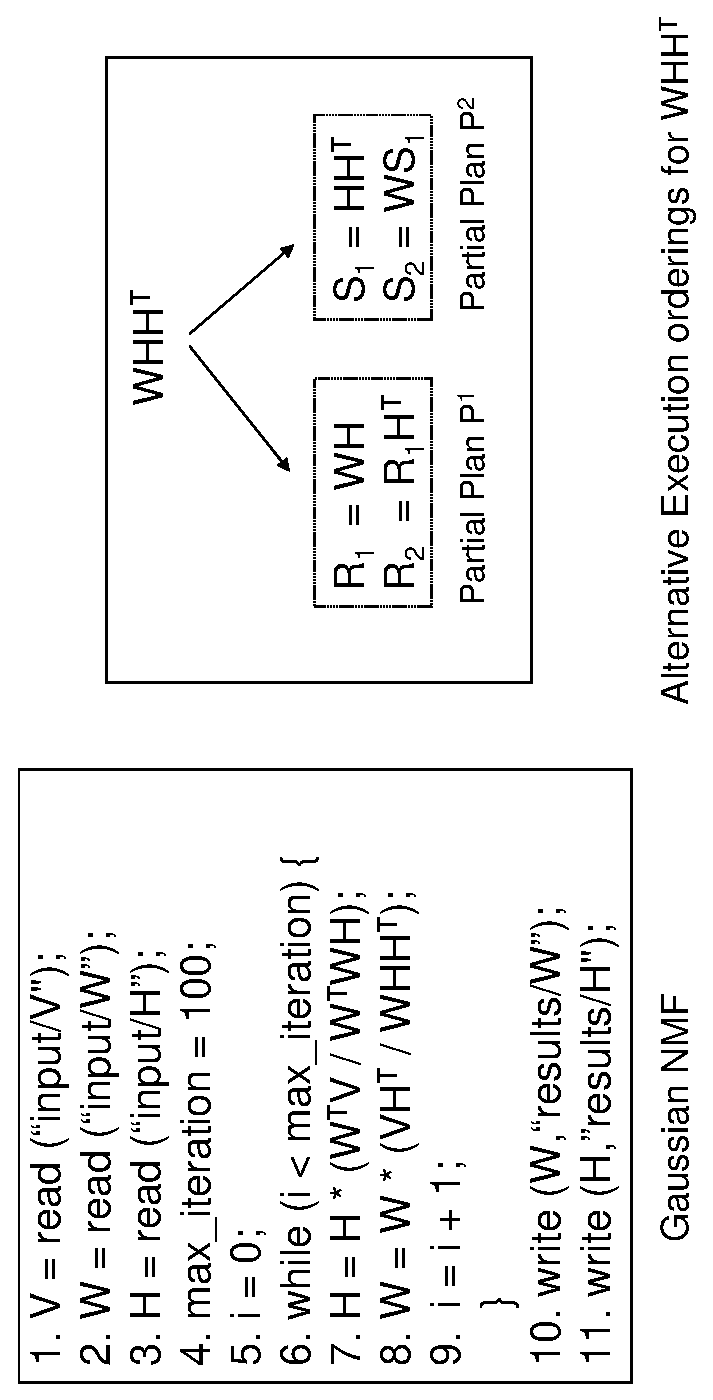
\includegraphics[angle=270,width=3.5in]{figures/gnmf.eps}
%\caption{Gaussian Non-Negative Matrix Factorization}
%\label{fig:gnmf}
%\end{figure}

Consider the expression $WHH^T$ in Step~8 of
Algorithm~\ref{algo:gnmf}. This expression can be
evaluated in one of two orders, $od1$: $(WH)H^T$ and $od2$: $W(HH^T)$. 
At first glance, picking the right order and performing this computation 
may seem straightforward, but the fact that matrix multiplication itself can be accomplished in 
multiple ways complicates matters.

Figure~\ref{fig:mmult2} and Figure~\ref{fig:mmult1} show two alternative MapReduce plans for matrix
multiplication (details of the two plans will be discussed in Section~\ref{sec:matrixmult}). The RMM
plan in Figure~\ref{fig:mmult2} implements a replication-based strategy in a single MapReduce job,
while the CPMM plan in Figure~\ref{fig:mmult1} implements a cross-product strategy that requires 2
MapReduce jobs. The choice of RMM vs CPMM is dictated by the characteristics of the matrices
involved in the multiplication. To compute $WHH^T$, we have to choose from a total of 8 plans: first
choose the order of evaluation, $od1$ or $od2$, and for the chosen order choose from RMM or CPMM for
each matrix multiplication. Instantiating the dimensionalities of the matrices reveals the need to
choose one plan over another. In the context of topic modeling, the number of topics $t$ is much
smaller than the number of documents $d$ and the number of words $w$. As a result, $od1$ will never
be selected as the evaluation order, since $WH$ produces a $d\times w$ large intermediate matrix
whereas $HH^T$ in $od2$ results in a $t\times t$ small matrix. When $d=10^7$, $w=10^5$ and $t=10$, H
is of medium size and the result of $HH^T$ is tiny. The replication based approach RMM performs very
well for both matrix multiplications. The best plan with $od2$ is to use RMM for $HH^T$ followed by
another RMM for the pre-multiplication with W.  Empirically, this plan is 1.5 times faster than the
second best plan of using CPMM followed by RMM. However, when $w$ is changed to $5\times 10^7$, size
of H increases 500 times. The overhead of replicating $H$ and $H^T$ makes RMM inferior to CPMM for
the computation of $HH^T$. On the other hand, the result of $HH^T$ remains to be a tiny matrix, so
the best plan to compute the pre-multiplication with W is still RMM. A cost model and a detailed
discussion on choosing between CPMM and RMM will be provided in Section~\ref{sec:matrixmult}.

%Note that while these optimizations are similar in spirit to join
%reordering and join method selection in relational database
%literature, applying them in the context of a declarative machine learning system on MapReduce enables unique opportunities for optimization.
%\end{example}

\customizedfig
{figures/mmult2.eps}
{RMM: Replication based Matrix Multiplication}
{fig:mmult2}
{2.6in}

\customizedfig
{figures/mmult1.eps}
{CPMM: Cross Product based Matrix Multiplication}
{fig:mmult1}
{2.4in}

As shown above, the choice of a good execution strategy depends 
significantly on data characteristics. 
Pushing this burden on programmers will have serious
implications in terms of scaling both development and execution time. 
This paper takes a step towards addressing this problem. 

\noindent {\bf Problem Statement}: Build a scalable declarative machine
learning system that
\begin{itemize}
\item exposes a declarative higher-level language for writing ML algorithms, thereby 
freeing the user from low-level implementation details and performance-tuning tasks. 
\item provides performance that scales to very large datasets and is comparable to hand-tuned implementations of individual algorithms.
\item covers a large class of ML and statistical algorithms whose computational cores are linear algebra primitives and iterative numerical optimization procedures. These include (but are not restricted to) linear statistical models, PCA, PageRank, Matrix Factorizations, and so on. 
\end{itemize}
 
The remainder of the paper is organized as follows. In Section~\ref{sec:overview}, we
present \systemml, in which ML algorithms are expressed in a higher-level language subsequently compiled and automatically parallelized to execute in Hadoop, an open source implementation of MapReduce. We then
describe the individual components of SystemML in Section~\ref{sec:arch}. 
We discuss the role of cost based optimization by showing two alternative execution plans for the expensive matrix multiplication operation.
We then present extensive experimental results
(Section~\ref{sec:experiments}) to demonstrate the scalability of \systemmltext\ and the effectiveness of the optimizations performed at various stages.

%To demonstrate the cost based optimization in SystemML, Section~\ref{sec:matrixmult} takes the expensive matrix multiplication operation as an example to discuss alternative execution plans and their associated cost models. 

%Our results demonstrate that our general-purpose system matches and at 
%times outperforms best published results based on hand-coded implementations of specific 
%algorithms.

%As background for the concepts presented in this paper, we provide a brief description of 
%MapReduce. Operationally, MapReduce consists of three phases: a \emph{Map phase} that 
%reads the data and produces a set of key-value pairs; a \emph{Shuffle phase} that sorts 
%all key-value pairs produced from the mappers by the key; and a \emph{Reduce phase} that 
%operates on all values associated with a given key and produces a new value for the same 
%key. Only the Map and Reduce phases are exposed to the user while the Shuffle phase is 
%typically internal to the platform. 
%For a more detailed description of MapReduce, the reader is referred to~\cite{mapreduce}. 
%We built our system on top of Hadoop~\cite{hadoop}, an open-source 
%implementation of MapReduce.

\begin{table*}[t]
\centering
\caption{Example operators in DML: $x_{ij}$, $y_{ij}$ and $z_{ij}$ are cells in matrices $X$, $Y$ and $Z$, respectively.} 
\label{tab:notation}
\begin{small}
\footnotesize
\begin{tabular}{|l|l|l|l|l|}
\hline
{\bf Algorithm~\ref{algo:gnmf}} & {\bf DML Statement}& {\bf Semantics} & {\bf HOP Notation} & {\bf LOP Notation}\\
\hline
$Z=X*Y$& \texttt{Z=X*Y} & cell-wise multiplication: $z_{ij}=x_{ij}*y_{ij}$ & $b(*): X, Y$ & $\grplop \rightarrow \binarylop(*)$\\
$Z=X/Y$& \texttt{Z=X/Y} & cell-wise division: $z_{ij}=x_{ij}/y_{ij}$ & $b(/): X, Y$ & $\grplop \rightarrow \binarylop(/)$\\
$Z=XY$& \texttt{Z=X\mmult Y} & matrix multiplication: $z_{ij}=\sum_{k}x_{ik}*y_{kj}$& $ab(\sum, *): X, Y$ & ($\rmmloptext$) or ($\mmcjlop \rightarrow \grplop \rightarrow \agglop(\sum)$)\\
$Z=X^T$& \texttt{Z=t(X)}& transpose: $z_{ij}=x_{ji}$ & $r(T): X$ & $\transloptext(t)$\\
& \texttt{Z=log(X)} & cell-wise logarithm: $z_{ij}=log(x_{ij})$  & $u(log): X$ & $\unarylop(log)$\\
%& \texttt{Z=X+0.5} &matrix-scalar addition: $z_{ij}=x_{ij}+0.5$ & $b(+): X, 0.5$ & $\unarylop(+)$\\
& \texttt{Z=rowSum(X)} & row-wise sums: $z_{i}=\sum_{j}x_{ij}$ & $au(\sum,\textit{row}): X$ & $\transloptext(\textit{row}) \rightarrow  \grplop \rightarrow \agglop(\sum)$\\
\hline
\end{tabular}
\BigCrunch
\end{small}
\end{table*}


%%
\section{\systemmltext\ Overview}
\label{sec:overview}
We now give an overview of \systemmlit. Figure~\ref{fig:arch} shows the overall 
architecture of \systemmlit\ that consists of four components. 
%Each component provides distinct functionality, thus enforcing modularity and enabling flexibility to extend \systemmlit\ to other runtime platforms.

\noindent {\bf Language:} Algorithms in \systemmlit\ are written in a high-level language 
called {\bf D}eclarative {\bf M}achine learning {\bf L}anguage (\dmlr). \dmlr\ exposes 
mathematical and linear algebra primitives on matrices that are natural to express a 
large class of ML algorithms, including linear models, PCA, PageRank, NMF etc. In addition, \dmlr\ supports 
control constructs such as \emph{while} and \emph{for} to write complex iterative 
algorithms. Through program analysis, \systemmlit\ breaks a \dmlr\ script into smaller 
units called {\it statement blocks}. Each statement block, separately, is optimized and executed by subsequent
components.

\noindent {\bf High-Level Operator Component (HOP):} The HOP component analyzes all the 
operations within a statement block and
chooses from multiple high-level execution plans. A plan is represented in
a HOP-Dag, a directed acyclic graph of basic operations (called \textit{hops}) over matrices and
scalars. Optimizations considered in this component include algebraic rewrites, selection of the physical representation for
intermediate matrices, and cost-based optimizations.

%The HOP component analyzes all the operations within a statement block and chooses from 
%multiple high-level execution plans (such as the alternative plans discussed in 
%Example~\ref{ex:gnmf}). Each execution plan is represented as a HOP-Dag, a directed 
%acyclic graph of basic operations (called \textit{hops}) over matrices and scalars. 
%Optimizations considered in this component include algebraic rewrites, selection of 
%physical representation for intermediate matrices and cost-based optimization.

\noindent {\bf Low-Level Operator Component (LOP):} The LOP component translates the 
high-level execution plans provided by the HOP component into low-level physical plans on MapReduce,
represented as LOP-Dags. Each low-level operator (\textit{lop}) in a LOP-Dag operates on
key-value pairs or scalars. The LOP-Dag is then compiled into one or more MapReduce jobs by packing
multiple lops into MapReduce jobs to keep the number of data scans small. We refer to this strategy
as {\em piggybacking}.
%The primary optimization performed in this component is piggybacking; i.e., deciding 
%which lops in a LOP-Dag can be grouped into a single MapReduce job. 

\noindent {\bf Runtime:} The runtime component executes the low-level plans obtained from 
the LOP component on Hadoop. The main execution engine in \systemmlit\ is a generic 
MapReduce job, which can be instructed to execute multiple lops inside it. A control 
module orchestrates the execution of different instances of the generic MapReduce job.
Multiple optimizations are performed in the runtime component; e.g., execution plans for 
individual lops are decided dynamically based on data characteristics such as sparsity of 
the input matrices.

%Note that the HOP component considers {\it logical} execution plans over matrices and scalars. Its optimizations are specific to operations on these high-level data types, such as deciding the correct execution order of a matrix multiplication chain (as discussed in Example~\ref{ex:gnmf}). In comparison, the LOP component captures operations specific to MapReduce over key-value pairs. As a result, the optimizations are aimed at translating the {\it physical} plans into efficient MapReduce operations. Each of the four components in \systemmlit\ provides distinct functionality, thus enforcing modularity and enabling flexibility to extend \systemmlit\ to other runtime platforms.

\sllsubfigures
{figures/arch.eps}
{\systemmltext \ Architecture}
{fig:arch}
{figures/example.eps}
{Evaluation of A=B*(C/D): conceptually, each key-value pair contains the index and the value of a cell in the matrix}
{fig:example}
{figures/programanalysis.eps}
{Program Analysis}
{fig:programanalysis}


Figure~\ref{fig:example} shows how a single DML statement \texttt{A=B*(C/D)} is processed in \systemmlit. The language expression consists of untyped variables and is translated into a HOP-Dag consisting of a cell-wise division hop and a cell-wise multiplication hop on matrices. A lower-level execution plan is then generated for this expression as shown in the LOP-Dag. Here, the {\it Cell-Wise Binary Divide} hop is translated into two lops -- a {\it Group} lop that sorts key-value pairs to align the cells from C and D; followed by the lop {\it Binary Divide on Each Group}. Finally, the entire LOP-Dag is translated into a single MapReduce job, where (a)~the mapper reads three inputs, (b)~all groupings are performed implicitly between the mapper and the reducer and (c)~the reducer performs the division followed by the multiplication.

%We now present the details of each component in \systemmlit.
%We describe each of the components in \systemmlit\ in more detail in the next section.


\section{\systemmltext\ Components}
\label{sec:arch}

\subsection{Declarative Machine learning Language (DML)} 
\label{sec:language}

%A popular tool amongst machine learning practitioners is R~\cite{R}.
%The language in R exposes a rich set of
%features including mathematical constructs such as linear algebra operations, 
%control structures such as while and for loops, function support including
%recursive functions and  object-oriented programming features. 
%While it provides the expressivity needed
%to implement a wide variety of ML algorithms, it is procedural in
%nature thereby precluding optimizations that consider 
%alternative plans such as those discussed in Example~\ref{algo:gnmf}.

\dmlr\ is a declarative language whose syntax closely resembles 
the syntax of R\footnote{R is prototypical for a larger class of such languages including
Matlab~\cite{matlab}}~\cite{R}. To enable more system generated optimization, \dmlr\ does not
provide all the flexibility available in R. However, this loss in flexibility results largely in
loss in programming convenience and does not significantly impact the class of ML algorithms that
are expressible in \dmlr.
%We begin by describing the features in \dmlr\ and then proceed to discuss the differences 
%with respect to R~\footnote{R is prototypical of a larger class of such languages 
%including Matlab~\cite{matlab}}. 
The GNMF algorithm (Algorithm~\ref{algo:gnmf}) is expressed in
\dmlr\ syntax in Script~\ref{scpt:gnmf}. We explain \dmlr\
constructs using this example.
\\ 
\begin{script}\label{scpt:gnmf}
GNMF\\
\footnotesize
\texttt{1:\ V=readMM("in/V", rows=1e8, cols=1e5, nnzs=1e10);\\
2:\ W=readMM("in/W", rows=1e8, cols=10);\\
3:\ H=readMM("in/H", rows=10, cols=1e5);\\
4:\ max\_iteration=20;\\
5:\ i=0;\\
6:\ \textbf{while}(i<max\_iteration)\{\\
7:\ \ \ H=H*(t(W)\mmult V)/(t(W)\mmult W\mmult H);\\
8:\ \ \ W=W*(V\mmult t(H))/(W\mmult H\mmult t(H));\\
9:\ \ \ i=i+1;\}\\
10:writeMM(W, "out/W");\\
11:writeMM(H, "out/H");}
\end{script}
\vspace*{0.1in}

\noindent {\bf Data Types:} \dmlr\ supports two main data types: matrices and 
scalars~\footnote{We treat vectors as a special case of matrices.}. Scalar 
data types supported are integer, double, string and logical. The cells in a matrix may 
consist of integer, double, string or logical values.

\noindent {\bf Statements:} A \dmlr\ program consists of a sequence of statements, with 
the default computation semantics being sequential evaluation of the individual 
statements. 

The following constructs are currently supported in \dmlr.

{\it Input/Output}: \concept{ReadMM} and \concept{WriteMM}
statements are provided for respectively reading and writing matrices from and to files. 
Optionally, in the \concept{ReadMM} statement,
the user can provide additional properties of the matrix
such as sparsity (number of non-zero entries or nnzs).

{\it Control Structures}: Control structures supported in \dmlr\
include the \concept{while} statement, \concept{for} statement and
\concept{if} statement. Steps~6-9 in Script~\ref{scpt:gnmf} show an
example \concept{while} statement.

{\it Assignment}: An \concept{assignment} statement 
consists of an expression and the result of which is assigned to a
variable - e.g., Steps~7 ,8 and 9 in Script~\ref{scpt:gnmf}. Note
that the assignment can be to a scalar or a matrix. 

%\begin{itemize}
%\item {\it Input/Output}: \concept{ReadMM} and \concept{WriteMM}
%statements are provided for respectively reading and writing, vectors
%or matrices, from and to files. Optionally, in the \concept{ReadMM} statement,
%the user can provide additional properties of the matrix or vector,
%such as dimensionality and sparsity (number of non-zero entries or nnzs).
%
%\item {\it Control Structures} : Control structures supported in \dmlr\
%include the \concept{while} statement, \concept{for} statement and
%\concept{if} statement. Steps~6-9 in Script~\ref{scpt:gnmf} show an
%example \concept{while} statement.
%
%\item {\it Assignment}: An \concept{assignment} statement 
%consists of an expression and the result of which is assigned to a
%variable - e.g., Steps~7,8 and 9 in Script~\ref{scpt:gnmf}. Note
%that the assignment can be to a scalar, vector or matrix. 
%\end{itemize}

%Table~\ref{tab:operators} lists the main types of operators supported
%in \dmlr\ along with a few examples for each type. The arithmetic
%operators extend naturally to matrices and vectors where the semantics
%is such that the operator is applied to the corresponding cells. For
%instance the expression C = \binaryop{A}{*}{B} will multiply the
%values in the corresponding cells in A and B and populate the
%appropriate cell in C with the result. Several internal functions,
%specific to particular data types, are
%supported. E.g., \concept{colSum} computes the sum of every column in
%a matrix and returns a vector, while \concept{t} computes the
%transpose of a matrix.

Table~\ref{tab:notation} lists several example operators allowed in expressions in \dmlr. 
The arithmetic operators $+,-,*,/$ extend naturally to matrices where the semantics is 
such that the operator is applied to the corresponding cells. For instance, the expression 
$Z=X*Y$ will multiply the values in the corresponding cells in $X$ and $Y$, and populate 
the appropriate cell in $Z$ with the result. Several internal functions, specific to 
particular data types, are supported -- e.g., \concept{rowSum} computes the sum of every 
row in a matrix and returns a column matrix (i.e., a vector), while \concept{t($\cdot$)} 
computes the transpose of a matrix.

\dmlr\ also allows users to define their own functions using the syntax {\textit 
{``function~~(arglist)~~body''}}. Here, the \textit{arglist} consists of a set of formal 
input and output arguments and the body is a group of valid \dmlr\ statements.

\noindent {\bf Comparison with R programming language:} As pointed out before, we have 
made some choices in the design of \dmlr\ to better enable system optimizations. For 
example, \dmlr\ does not support \emph{object oriented features}, \emph{advanced data 
types} (such as lists and arrays) and \emph{advanced function support} (such as accessing 
variables in the caller function and further up in the call-stack). Besides these advanced 
features for programming convenience, R also supports extensive \emph{graphical 
procedures} that are clearly beyond the scope of \dmlr.

%\emph{[[Note: I also suggest that at the end of the paper
%in the discussion section we have a paragraph on ``Revisiting Design Choices of \dmlr\ ``.]]}


\noindent {\bf Program Analysis:}
We now describe the sequence of steps a \dmlr\ script goes through to generate a parsed 
representation. Figure~\ref{fig:programanalysis} shows the result of program analysis for 
Script~\ref{scpt:gnmf}.

{\it Type Assignment}: The first step is to assign data types to
each variable in the \dmlr\ script. For instance, \concept{ReadMM}
statements (Steps~1-3) are used to type V, W and H as matrices, while \concept{Assignment} 
statements (Steps~4-5) are used to identify $max\_iteration$ and $i$ as scalar variables. 
%This information is then propagated through the rest of the program.

{\it Statement Block Identification}: As control constructs (such as \concept{while}) and 
\concept{functions} break the sequential flow of a \dmlr\ program, they naturally divide 
the program into \textit{statement blocks}. Each statement block consists of consecutive 
\concept{Assignment}, \concept{ReadMM} and \concept{WriteMM} statements, as the operations 
involved in these statements can be collectively optimized. 
Figure~\ref{fig:programanalysis} illustrates our example algorithm broken down into three 
statement blocks ($SB_1, SB_2$ and $SB_3$).

%\item {\it Live Variable Analysis}. Notice how variables may be
%updated-in-place in a \dmlr\ program. E.g., in Step~8, the variable W
%is both read and written in the same statement. Since this statement
%appears within a \concept{while} loop, W may either refer to the
%output of Step~2 (for the first iteration) or Step~8 in the previous
%iteration (for subsequent iterations). Furthermore, we need to decide
%what variables need to be passed across statement blocks. Therefore,
%we perform live-variable analysis~\footnote{This is similar to the
%classic data flow analysis typically performed by compilers in
%programming languages} on the program to connect each variable use
%with the previous write for that variable. For each statement block,
%we also identify the variables that will be required from previous
%statement blocks ({\it Live Variables In}) and the variables that will
%be output by the current statement block ({\it Live Variables
%Out}). The results of live variable analysis are shown in
%Figure~\ref{fig:programanalysis}.

{\it Live Variable Analysis}: The goal of this step is twofold:
(a)~Connect each variable use with the immediately preceding write(s)
for that variable across different evaluation paths. For example,
variable W used in Step~7 refers to the output of Step~2 for the
first iteration of the loop and Step~8 for second iteration onwards. (b)~For each statement block, identify the variables that will be required from previous
statement blocks ({\it Live Variables In}) and the variables that will
be output by the current statement block ({\it Live Variables Out}). 
The results of live variable analysis are shown in Figure~\ref{fig:programanalysis}.




%{\tt Sekar, you need to explain: program, statement block, variable analysis, damn across statement blocks.}


\subsection{High-Level Operator Component (HOP)}
\label{sec:hops}
\begin{table*}[t]
\centering
\caption{Example hops in SystemML: $x_{ij}$, $y_{ij}$ are cells in matrices $X$, $Y$, respectively.}
\label{tab:hop}
\begin{small}
\footnotesize
\begin{tabular}{|l|l|m{3.2in}|l|}
\hline
{\bf HOP Type} & {\bf Notation} & {\bf Semantics} & {\bf Example in Table~\ref{tab:notation}} \\
\hline
{\em Binary} &$b(op): X, Y$  & for each $x_{ij}$ and $y_{ij}$, perform $op(x_{ij}, y_{ij})$, where $op$ is $*, +, -, /$ etc. & $b(*): X, Y$ \\ \hline
{\em Unary} &$u(op): X$ & for each $x_{ij}$, perform $op(x_{ij})$, where $op$ is $log$, $sin$ etc. & $u(log): X$\\ \hline
{\em AggregateUnary}& $au(aggop, dimension): X$ & apply $aggop$ for the cells in dimension, where $aggop$ is $\sum$, $\prod$ etc, and $dimension$ is  
$row$ (row wise), $col$ (column wise) or $all$ (the whole matrix). & $au(\sum,row): X$\\ \hline
{\em AggregateBinary}& $ab(aggop, op): X, Y$ & for each $i,j$, perform $aggop(\{op(x_{ik}, y_{kj})| \forall k\})$, where $op$ is $*, +, -, /$ etc, and $aggop$ is 
$\sum$, $\prod$ etc. & $ab(\sum, *): X, Y$ \\  \hline
{\em Reorg} & $r(op): X$ & reorganize elements in a matrix, such as transpose ($op=T$). & $r(T): X$ \\ \hline
{\em Data} & $data(op): X$ & read ($op=r$) or write ($op=w$) a matrix. & \\ 
\hline
\end{tabular}
\end{small}
\SmallCrunch
\end{table*}

The HOP component takes the parsed representation of a statement block as input, and produces a HOP-Dag representing the data flow. 
%We first describe the hops available in \systemmltext\ along with
%their semantics, and then describe the construction of HOP-Dag.


\customizedfigInCol
{figures/hoplop.eps} 
{HOP-Dag, LOP-Dag and Runtime of the while Loop Body in Figure~\ref{fig:programanalysis}}
{fig:hoplop}
{5in}

\noindent{\bf Description of hops:} 
Each hop in the HOP-Dag has one or more input(s), performs an operation or transformation, 
and produces output that is consumed by one or more subsequent hops. Table~\ref{tab:hop} 
lists some example hops supported in \systemmltext\ along with their 
semantics\footnote{Table~\ref{tab:hop} describes the semantics of hops in terms of 
matrices. Semantics of hops for scalars are similar in spirit.}. In addition, the instantiation of hops from the \dmlr\ parsed representation is exemplified in Table~\ref{tab:notation}. 
Consider the matrix multiplication \texttt{Z=X\mmult Y} as an instance, an {\em 
AggregateBinary} hop is instantiated with the binary operation $*$ and the aggregate operation $\sum$. The semantics of this hop instance, denoted by $ab(\sum,*)$, is to compute, $\forall i,j, \sum_k ({x_{i,k} * y_{k,j}})$. 


%Consider the cell-wise multiplication \texttt{Z=X*Y} as an instance, a {\em Binary} hop is instantiated with binary operation $*$, and $X$ and $Y$ as operands. The semantics of this binary hop is to compute $x_{i,j} * y_{i,j}$ for every pair of corresponding cells in the two matrices. For the more complex matrix multiplication \texttt{Z=X\mmult Y}, an {\em AggregateBinary} hop is instantiated with the binary operation $*$ and the aggregate operation $\sum$. The semantics of hop instance, denoted by $ab(\sum,*)$, is to compute, $\forall i,j, \sum_k ({x_{i,k} * y_{k,j}})$. 

%To understand the instantiation of hops from the \dmlr\ parsed representation,
%let us consider the cell-wise division of matrices $C$ and $D$ shown in
%Figure~\ref{fig:example}. a {\em Binary} hop is instantiated with
%binary operation $/$, and $C$ and $D$ as operands. The semantics of this
%binary hop is such that it computes $c_{i,j} / d_{i,j}$ for every
%pair of corresponding cells in the two matrices. For a more complex hop 
%such as {\em AggregateBinary}, let us consider the  matrix multiplication 
%$W \mmult H$ in Script~\ref{scpt:gnmf}. For this purpose an
%{\em AggBinary} hop is instantiated
%with the binary operation $*$ and the aggregate operation $+$. 
%
%Data hops can be transient or persistent with respect to the lifetime of a script.


\noindent{\bf Construction of HOP-Dag:} 
The computation in each statement block is represented as one HOP-Dag~\footnote{Statement blocks for control structures such as {\it while} loops have additional HOP-Dags, e.g. for representing predicates.}. Figure~\ref{fig:hoplop}(a) shows the HOP-Dag for the body of the \textit{while} loop statement block in Figure~\ref{fig:programanalysis} constructed using the hops in Table~\ref{tab:hop}. Note how multiple statements in a statement block have been combined into a single HOP-Dag. The HOP-Dag need not be a connected graph, as shown in Figure~\ref{fig:hoplop}(a).

The computation \texttt{t(W)\mmult W} in the statement block is represented 
using four hops -- a {\it data(r):$W$} hop that reads $W$ is fed into a Reorg hop 
{\it r($T$)} to perform the matrix transposition, which is then fed, along with the {\it 
data(r):$W$} hop, into an AggregateBinary hop {\it $ab(\sum,*)$} to perform the matrix 
multiplication. 
%Note that a HOP-Dag does not have to be connected as shown in 
%Figure~\ref{fig:hoplop}(a).

%The hop {\it data(r):$W$} feeds into the Reorg hop {\it r($T$)}, which in turn feeds into 
%the AggregateBinary hop {\it $ab(\sum,*)$} together with the {\it data(r):$W$} hop to 
%represent the \texttt{t(W)\mmult W} part of the statement block. Note that a HOP-Dag does 
%not have to be connected as shown in Figure~\ref{fig:hoplop}(a).

The grayed \textit{data(r)} hops represent the live-in variables for matrices
$W$, $H$, and $V$, and the scalar $i$ at the beginning of an
iteration\footnote{The max\_iteration variable is used in the HOP-Dag
for the \concept{while} loop predicate.}. The grayed \textit{data(w)} hops
represent the live-out variables at the end of an iteration that need
to be passed onto the next iteration. These data hops -- which are
transient -- implicitly connect HOP-Dags of different statement blocks
by mapping the transient \textit{data(w)} hops (sinks) of
one statement block to the transient \textit{data(r)} hops (sources) of the next statement 
block, or the next iteration of the \concept{while} loop.

%\begin{figure}[t]
%\center
%{\includegraphics[width=2.6in]{figures/hopsdag.eps}}
%\caption{HOPDag for While Loop Body in Figure~\ref{fig:programanalysis}.}
%\label{fig:hopdag}
%\end{figure}


\subsection{Low-Level Operator Component (LOP)}
\label{sec:lops}
The LOP component translates HOP-Dags into corresponding low-level physical execution 
plans (or LOP-Dags). In this section, we detail the low-level operators (lop) that 
describe individual operations over key-value pairs and show how a LOP-Dag is constructed 
from a HOP-Dag. We also present a greedy \emph{piggybacking heuristic} for packaging lops 
into small number of MapReduce jobs.

\noindent {\bf Description of lops:} Lops represent basic operations in a MapReduce environment. Each lop takes one or more sets of key-value pairs as
input and generates one set of key-value pairs as output that can be consumed by one or more lops. 
Example lops\footnote{Lops over scalars are omitted in the interest of space.} are provided in Table~\ref{tab:lopproperties}.
%For example, the \grplop\ takes in multiple sets of key-value pairs and groups the values based on their keys. The \binarylop\  

\noindent{\bf Construction of LOP-Dags:} A HOP-Dag is processed in a bottom-up fashion to 
generate the corresponding LOP-Dag by translating each hop into one or more lops.
Figure~\ref{fig:lopsexample} describes the translation of a \textit{Binary} hop to the corresponding
lops for the expression \texttt{C/D} (Figure~\ref{fig:example}). At the bottom, each of the
two \datalop \ lops returns one set of key-value pairs for the input matrices, conceptually, one
entry for each cell in the individual matrices. (In practice, as will be described in
Section~\ref{sec:blocking}, \datalop\ lop typically returns multiple cells for each key where the
number of cells is determined by an appropriate blocking strategy.) A \grplop\ then groups or sorts
the key-value pairs from the two inputs based on their key. Each resulting group is then passed on
to a \binarylop\ lop to perform the division of the corresponding cell-values. Other example
translations of hops to lops are provided in Table~\ref{tab:notation}.

Figure~\ref{fig:hoplop}(b) shows the generated LOP-Dag for the ``H Assignment" part of the 
HOP-Dag in Figure~\ref{fig:hoplop}(a). Note that the \textit{AggregateBinary} hop for 
matrix multiplication can be translated into different sequences of lops (see the last 
column of the 3rd row in Table~\ref{tab:notation}). In our example of 
Figure~\ref{fig:hoplop}(b), $\mmcjlop \rightarrow \grplop \rightarrow \agglop(\sum)$ is 
chosen for \texttt{t(W)\mmult V} and \texttt{t(W)\mmult W},  
and \rmmlop\ is chosen for multiplying the result of (\texttt{t(W)\mmult W}) with \texttt{H}.

\noindent{\bf Packaging a LOP-Dag into MapReduce jobs:}
Translating every lop to a MapReduce job, though straightforward, will result in multiple 
scans of input data and intermediate results. If, however, multiple lops can be packaged 
into a single MapReduce job, the resulting reduction in scans may result in an improvement 
in efficiency. Packing multiple lops into a single MapReduce job requires clear 
understanding of the following two properties of lops:

\emph{Location}: whether the lop can be performed in Map, Reduce, either or both phases. 
Note that the execution of certain lops, such as \grplop, spans both Map and Reduce 
phases.

\emph{Key Characteristics}: whether the input keys are required to be grouped, the output 
keys produced are grouped, and whether the lop generates different output keys. 

These properties for the individual lops are summarized in Table~\ref{tab:lopproperties}. Algorithm~\ref{algo:piggybacking} describes the greedy {\it piggybacking algorithm} that packs the lops in a LOP-Dag into a small number of MapReduce jobs. The nodes in a given LOP-Dag are first topologically sorted, and then partitioned into multiple lists based on their execution location property. Note that the nodes within each list are in topologically sorted order. The approach then iteratively assigns the lops to one or more MapReduce job(s). During each iteration, it allocates a new MapReduce job and assigns lops first to the Map phase, then assigns lops that span the Map and Reduce phases, and finally assigns lops to the Reduce phase. This assignment is carried out by invoking the method $addNodesByLocation$. 

%A given lop node is assigned to a job for its execution only after all of its descendant lops in the LOP-Dag have already been assigned (Line 17). Since the lops with execution location $MapAndReduce$ perform an implicit sort, they are assigned to jobs one at a time (Line 21). Group lops (with execution location $MapAndReduce$) are added to the reduce phase provided the same MapReduce job has been assigned a descendant group lop and that none of the intermediate lops between the two group lops alter the keys (Line 24). 

Lop nodes with
execution locations of $Map$ or $MapOrReduce$ can be assigned to the Map phase provided their
descendants in the LOP-Dag have already been assigned. 
Note that the descendants of a given lop $p$ are the ones that have a directed path to $p$, and they appear prior to $p$ in a topological sort. 
When no more lops can be added to the Map phase, we proceed to add lops that span the Map and Reduce phases, ensuring that another
descendant with execution location $MapAndReduce$ will not be assigned to the same job. Finally,
lops with the execution locations of $MapOrReduce$ and $Reduce$ are directly added to the Reduce
phase of the job provided their descendants have already been assigned. Group lops (with execution
location $MapAndReduce$) can be added to the reduce phase provided the same MapReduce job has been
assigned a descendant group lop and that none of the intermediate lops between the two group lops
alter the keys. 
For example, consider the five lops shown as dotted boxes in Figure~\ref{fig:hoplop}(b). 
The first {\em group} lop is assigned to span Map and Reduce phases of the job. 
Remaining two {\em group} lops are executed in the Reduce phase because the $aggr.(+)$ and $binary(/)$ lops do not alter the keys.
%Since $binary(/)$ lop does not alter the keys, the subsequent {\em group} lop is assigned to the Reduce phase. 
Therefore, the entire LOP-Dag is packed into just five MapReduce jobs (see Figure~\ref{fig:hoplop}(c)). 
The job number is shown next to each lop in Figure~\ref{fig:hoplop}(b). Overall runtime complexity of our piggybacking strategy is quadratic in LOP-Dag size.
While Pig~\cite{pig} also makes an effort to pack multiple operators into MapReduce jobs, their approach is not readily applicable for complex linear algebraic operations.

%Note that Pig~\cite{pig} also packs several database-related operators into MapReduce jobs. 
%However, their strategy is fairly simple when compared to our piggybacking approach that aims to reduce the number of resulting jobs.
%Similarly to SystemML's piggybacking, Pig~\cite{pig} also assigns multiple physical operators to different phases of a MapReduce job, but for database-like selection, aggregation and join operations. 


%Lop nodes with
%execution locations of $Map$ or $MapOrReduce$ can be assigned to the Map phase provided their
%descendants in the LOP-Dag have already been assigned. When no more lops can be added to the Map
%phase, we proceed with adding lops that span the Map and Reduce phases, ensuring that another
%descendant with execution location $MapAndReduce$ will not be assigned to the same job. Finally,
%lops with the execution locations of $MapOrReduce$ and $Reduce$ are directly added to the Reduce
%phase of the job provided their descendants have already been assigned. Group lops (with execution
%location $MapAndReduce$) can be added to the reduce phase provided the same MapReduce job has been
%assigned a descendant group lop and that none of the intermediate lops between the two group lops
%alter the keys. For example in Figure~\ref{fig:hoplop}(b), the {\em group} lop that is marked with a
%dotted circle is assigned to the Reduce phase as the $binary(/)$ lop underneath it does not alter
%the keys. Therefore, the entire LOP-Dag can be packed into just five MapReduce jobs as shown in
%Figure~\ref{fig:hoplop}(c). The job number is shown next to each lop in Figure~\ref{fig:hoplop}(b). 
%Similar to SystemML's piggybacking, Pig~\cite{pig} also assigns multiple physical operators to 
%different phases of a MapReduce job, but for database-like selection, aggregation and join operations. 

%\reminder{Amol and Shirish. Explain topological sort in algorithm; is it deterministic, i.e. if I run it again w/ same LOP-Dag, will i get same instructions? Runtime program instructions in line 2 are not explained. Inconsistency: Location is called execution phase in Table III. Table III Data lop: can be in Map or Reduce?? Don't think so. Fix ``scalar'' in Table III.}


\begin{table*}[]
\caption{Example lops in SystemML: $\{\langle(i,j), x_{ij}\rangle\}$ is the conceptual key-value representation of Matrix $X$}
\label{tab:lopproperties}
\footnotesize
\begin{tabular}{|l|l|l|l|}
\hline
\textbf{LOP Type} & \textbf{Description} & \textbf{Execution Location} & \textbf{Key Characteristics} \\ \hline
\datalop & input data source or output data sink, in key value pairs $\{\langle(i,j), x_{ij}\rangle\}$ & Map or Reduce& none \\ \hline
%\scalarlop &operate on each value, $\{\langle(i,j), x_{ij}\rangle\}$ $\Mapsto$ $\{\langle(i,j), op(x_{ij})\rangle\}$ & Map or Reduce & none \\ \hline
\scalarlop &operate on each value with an optional scalar, $\{\langle(i,j), x_{ij}\rangle\},s$ $\Mapsto$ $\{\langle(i,j), op(x_{ij},s)\rangle\}$
& Map or Reduce & none \\ \hline
\translop & transform each key, $\{\langle(i,j), x_{ij}\rangle\}$ $\Mapsto$ $\{\langle trans(i,j), x_{ij}\rangle\}$
& Map or Reduce & keys changed   \\ \hline
\grplop & groups values by the key, $\{\langle(i,j), x_{ij}\rangle\},\{\langle(i,j), y_{ij}\rangle\}...$ $\Mapsto$ $\{\langle(i,j), \{x_{ij}, y_{ij}...\}\rangle\}$ 
&  Map and Reduce & output keys grouped \\ \hline
\binarylop & operate on two values with the same key,  $\{\langle(i,j), \{x_{ij}, y_{ij}\}\rangle\}$ $\Mapsto$ $\{\langle(i,j), op(x_{ij}, y_{ij})\rangle\}$ 
& Reduce & input keys grouped \\ \hline
\agglop & aggregate all the values with the same key, $\{\langle(i,j), values\rangle\}$ $\Mapsto$ $\{\langle(i,j), agg(values)\rangle\}$ 
& Reduce & input keys grouped \\ \hline
\mmcjlop &cross product computation in the CPMM matrix multiplication, 
& Map and Reduce & none \\ 
& $\{\langle(i,k), x_{ik}\rangle\},\{\langle(k,j), y_{kj}\rangle\}$ $\Mapsto$ $\{\langle(i,j), op(x_{ik}, y_{kj})\rangle\}$& & \\ \hline
\rmmlop &RMM matrix multiplication,   
& Map and Reduce & none \\ 
& $\{\langle(i,k), x_{ik}\rangle\},\{\langle(k,j), y_{kj}\rangle\}$ $\Mapsto$ $\{\langle(i,j), agg(\{op(x_{ik}, y_{kj})\})\rangle\}$& &\\ \hline
%%partial\_aggregate\_lop & Map or Reduce & changes indices \\ \hline
\end{tabular}
\SmallCrunch
\end{table*}

\eat{
\begin{algorithm}
\begin{scriptsize}
\begin{algorithmic}[1]
\STATE SortedNodes $\leftarrow$ TopologicalSort(LOPDag)
\STATE ReadyNodes $\leftarrow$ Leaf Nodes in SortedNodes
\WHILE{(Nodes remain to be assigned)}
\STATE Create a new MapReduce job $MR_i$
\STATE \COMMENT{Assign lops to Mapper based on location property}
\FOR{($n \in ReadyNodes$ is of type \scalarlop, \translop\ or \datalop)} 
\STATE Assign $n$ to $MR_i$
\STATE Remove $n$ from ReadyNodes and add children of $n$ to ReadyNodes.
\ENDFOR
\STATE \COMMENT{Assign lops to Map and Reduce based on location property}
\FOR{($n \in $ ReadyNodes is of type \grplop, \mmcjlop\ or \rmmlop)} 
\STATE Assign $n$ to $MR_i$ if $\not \exists n_1$ assigned to $MR_i$ such that $n_1$ is an ancestor of $n$ with lop type \grplop, \mmcjlop\ or \rmmlop.
\STATE Remove $n$ from ReadyNodes and add children of $n$ to ReadyNodes.
\ENDFOR
\STATE \COMMENT{Assign lops to Reduce based on location property}
\FOR{($n \in $ ReadyNodes is of type \binarylop, \agglop\ or \grplop)}
\STATE \COMMENT{Take Key Characteristics into account; input needs to be grouped}
\STATE Assign $n$ to $MR_i$, if $\exists n_1$ assigned to $MR_i$, $n_1$ is an ancestor of $n$ and of type \grplop\ and $\not \exists$ \translop\ child of $n_1$ assigned to $MR_i$. 
\STATE Remove $n$ from ReadyNodes and add children of $n$ to ReadyNodes.
\ENDFOR
\ENDWHILE
\end{algorithmic}
\caption{Piggybacking : Grouping lops that can be evaluated together in a single MapReduce job}
\label{algo:piggybacking}
\end{scriptsize}
\end{algorithm}
}


\eat{
\begin{algorithm}
\begin{scriptsize}
\begin{algorithmic}[1]
\STATE Input:  LOP-Dag
\STATE Output: Runtime program instructions ($prog$)
\STATE \COMMENT{Group nodes based on execution location and then topologically sort each group} 
\STATE [MapN, MapOrReduceN, MapAndReduceN, ReduceN] $\leftarrow$ TopoSort(LOP-Dag);
\WHILE{(Nodes in LOP-Dag remain to be assigned)}
\STATE Job $\leftarrow$ create a new MapReduce job;
\STATE \COMMENT{Iteratively assign lops to the Mapper}
\STATE addNodesByLocation(MapN $\cup$ MapOrReduceN, Map, Job);
\STATE \COMMENT{Assign lops that span Mapper and Reducer}
\STATE addNodesByLocation(MapAndReduceN, MapAndReduce, Job);
\STATE \COMMENT{Iteratively assign lops to the Reducer}
\STATE addNodesByLocation(MapOrReduceN $\cup$ MapAndReduceN $\cup$ ReduceN, Reduce, Job);
\STATE inst $\leftarrow$ getInstructions(Job);
\STATE add inst to $prog$;
\ENDWHILE
\STATE ~
\STATE \COMMENT{Method to add nodes that are ready to be assigned for a specific execution location}
\STATE Method: addNodesByLocation ( S, loc, Job )
\WHILE{(true)}
\STATE  readyNodes = \{ \};
	\WHILE {( S is not empty )} 
	\STATE n $\leftarrow$ S.next();
		\IF{(n is not yet assigned and all parents of n have been assigned)} 
			\IF{(loc is Map )}
			\STATE add n to readyNodes;
			\ENDIF 
			\IF{(loc is MapAndReduce )}
				\IF{(n does not have a descendant lop with execution location MapAndReduce in readyNodes and Job)}
				\STATE add n to readyNodes;
				\ENDIF
			\ENDIF
			\IF{(loc is Reduce)} 
				\IF{(n is not a group lop)}
				\STATE add n to readyNodes;
				\ENDIF
				\STATE \COMMENT{Add group lops to the same job if the keys are already sorted}
				\IF{(n is a group lop \& n has a descendant group lop in readyNodes or Job \& none of the lops between these two group lops alter keys)}
				\STATE add n to readyNodes; 
				\ENDIF
			\ENDIF
		\ENDIF
	\ENDWHILE
	\IF{(readyNodes is empty)}
	\STATE break;
	\ENDIF
	\IF{(loc is Map)}
	\STATE addNodes(Job.Map, readyNodes);
	\ENDIF
	\IF{(loc is MapAndReduce)}
	\STATE addNodes(Job.MapAndReduce, readyNodes);
	\ENDIF
	\IF{(loc is Reduce)}
	\STATE addNodes(Job.Reduce, readyNodes);
	\ENDIF
\ENDWHILE
\end{algorithmic}
\caption{Piggybacking : Grouping lops that can be evaluated together in a single MapReduce job}
\label{algo:piggybacking}
\end{scriptsize}
\end{algorithm}
}

\customizedfig
{figures/LopsExample.eps}
{Translating hop to lop for expression $C/D$ from Figure~\ref{fig:example}}
{fig:lopsexample}
{2in}

\begin{algorithm}
\begin{scriptsize}
\begin{algorithmic}[1]
\STATE Input:  LOP-Dag
\STATE Output: A set of MapReduce Jobs($MRJobs$)
\STATE [$N_{Map}, N_{MapOrRed}, N_{MapAndRed}, N_{Red}$] = TopologicalSort(LOP-Dag);
\WHILE{(Nodes in LOP-Dag remain to be assigned)}
\STATE Job $\leftarrow$ create a new MapReduce job;
\STATE addNodesByLocation($N_{Map} \cup N_{MapOrRed}$, Map, Job);
\STATE addNodesByLocation($N_{MapAndRed}$, MapAndReduce, Job);
\STATE addNodesByLocation($N_{MapOrRed} \cup N_{MapAndRed} \cup N_{Red}$, Reduce, Job);
\STATE add Job to $MRJobs$;
\ENDWHILE
\STATE ~
%\STATE \COMMENT{Method to add nodes that are ready to be assigned for a specific execution location}
\STATE {\bf Method:} {\it addNodesByLocation ( S, loc, Job )}
\WHILE{(true)}
\STATE  Z $\leftarrow \phi$
\WHILE {( $S$ is not empty )} 
	\STATE $n$ $\leftarrow$ $S$.next()
	\IF{($n$ is not yet assigned and all descendants of $n$ have been assigned)} 
		\IF{($loc$ is Map )}
			\STATE add $n$ to Z
		\ELSIF{($loc$ is MapAndReduce )}
			\STATE add $n$ to Z if n does not have any descendant lop in Z and Job whose location is MapAndReduce 
		\ELSIF{($loc$ is Reduce)} 
			\STATE add $n$ to Z if $n$ is not a group lop
			\STATE if $n$ is a group lop: add $n$ to Z only if $n$ has a descendant group lop in Z or Job \& none of the lops between these two group lops alter keys
		\ENDIF
	\ENDIF
\ENDWHILE
\STATE break if Z is empty
\STATE add Z to $Job$.Map, $Job$.MapAndReduce, or $Job$.Reduce, based on $loc$
\ENDWHILE
\end{algorithmic}
\caption{Piggybacking : Packing lops that can be evaluated together in a single MapReduce job}
\label{algo:piggybacking}
\end{scriptsize}
\end{algorithm}

\eat{
The LOPDag is processed in a bottom-up fashion using a greedy heuristic that exploits the 
above properties. Figure~\ref{fig:piggybacking} shows how the computation of H is achieved 
using 5 MapReduce jobs. For instance, the computation $t(W) \mmult W$ is performed in a 
single MapReduce job, with the transform operator in the map phase and the matrix 
multiplication (\rmmlop) in the map, shuffle and reduce phases.
}

%{\noindent{\bf {Matrix Multiplication Algorithms}} Assume two blocked matrices $A$ and $B$ with 
%$M_b \times K_b$ blocks in $A$ and $K_b \times N_b$
%blocks in $B$. The matrix multiplication computation at the block level corresponds to $C_{i,j}
%=\sum_k{ A_{i,k} \times B_{k,j}}$.

\eat{
Figure~\ref{fig:mmult2} illustrates the replication based matrix multiplication approach 
(RMM), which requires only one MapReduce job. The LOPDag for this execution plan contains 
a single \rmmloptext\ lop, which is implemented in the MapAndReduce phase of the generic 
MapReduce job. In this approach, each reducer computes one or more result blocks, i.e., 
$C_{i,j}$'s, and the mappers send the required data to the reducers. Since each block 
$A_{i,k}$ contributes to the computation of several result blocks ($C_{i,0}$, $C_{i,1}$, 
$\ldots$, $C_{i, N_b-1}$), the mapper sends $N_b$ copies of $A_{i,k}$ to the corresponding 
reducers. Similarly, $M_b$ copies of $B_{k,j}$ are sent to the corresponding reducers. 
Within each reducer, since all the required blocks for computing $C_{i,j}$ are available, 
the result is computed by performing block-based matrix multiplication followed by 
aggregation.

Figure~\ref{fig:mmult1} demonstrates the Cross Product based approach for matrix
multiplication. CPMM is represented in LOPDags as a sequence of three lops
-- \mmcjloptext, \grploptext\ and \aggloptext, and requires 2 MapReduce jobs for execution. For
instance, Figure~\ref{fig:piggybacking} shows a CPMM evaluation for the computation of $W^TW$. In
the Map phase of the first MapReduce job for CPMM, the two input matrices A and B are read. In the
MapAndReduce phase, \mmcjloptext\ groups input blocks $A_{i,k}$'s and $B_{k,j}$'s by the common key
$k$ and performs a cross product to compute $C^k_{i,j}=A_{i,k}B_{k,j}$. These results are
passed along to the next MapReduce job by the Reduce phase. In the second MapReduce job, the Map
phase reads in these intermediate results. The \grploptext\ lop is evaluated in the MapAndReduce
phase to group all the $C^k_{i,j}$'s by the key $(i,j)$. Finally, in the Reduce phase,
the \aggloptext\ lop computes $C_{i,j}=\sum_k{C^k_{i,j}}$.
}

%We topologically sort the Lop DAG such that each child node appears before its parent node in the
%sorted order.  Next, we iteratively process the sorted DAG starting with the leaf nodes. We maintain
%a list of queued nodes and a list of execution nodes.  The list of queued nodes represents Lop nodes
%that cannot be processed during that iteration.  The list of execution nodes represents Lop nodes
%that can be processed during that iteration. Both lists are cleared at the start of each iteration.
%During each iteration, unprocessed Lop nodes whose child nodes are not queued are added to the list
%of execution nodes depending on some criteria. A Lop node of type Scalar is added to the list of
%execution nodes provided all its inputs are either ready or in the list of execution nodes.  Lop
%nodes of other types are added depending on whether or not they can be added to a Generic Map-Reduce
%job given their child nodes in the list of execution nodes.  A Lop node of type MapOrReduce or
%MapOrReduceBreaksAlignment can always be added to the list as its computation can be piggybacked in
%the mapper or the reducer.  A Lop node of type ReduceOnly requires that there not be a child node in
%the list that needs a reduce operation and it can be added provided it does not have a child node of
%type ReduceOnly in the list.  A Lop node of type AlignedReduce can always be piggybacked with a Lop
%of type ReduceOnly provided it does not have a child node of type MapOrReduceBreaksAlignment
%proceeding the Lop of type ReduceOnly.  A node that cannot be added to the list of execution nodes
%is added to the list of queued nodes.  For a queuedNode with two inputs for which one input is in
%the list of queued nodes, the non-queued input node, it child nodes in the list of execution nodes,
%and the parents of these child nodes, are queued. These will be processed in the next iteration.
%These heuristic strategies ensure that we pack as many Lops into a Map-Reduce job as possible
%thereby reducing the number of Map-Reduce jobs needed at runtime.  The list of execution nodes at
%the end of an iteration are then mapped into a list of one or more instructions, instructions being
%of type SimpleInstructions and MapReduceInstructions. In the case of SimpleInstructions, results of
%intermediate computations are managed through additional SimpleInstructions that allow for the
%creation, writing, and deletion of temporary variables when they are no longer needed.  In the case
%of MapReduceInstructions, Map-Reduce jobs that need to generate intermediate results are again
%managed using temporary directories that need to be deleted when they are no longer needed. The
%translator generates SimpleInstructions for file deletions to handle such cases.  This process
%continue iteratively until the entire Lop DAG is processed.

%{\tt The following text needs to be moved after runtime}

%{\tt Lops to Runtime Translation}

%The Runtime layer provides a small number of generic Map-Reduce jobs and a control program capable
%of executing small scale computations (such has scalar computations) outside of the Map-Reduce
%infrastructure.

%The Lops to Runtime translator processes the Lops DAG for each Statement Block to
%produce one or more instructions.  These instructions can be of two types - SimpleInstructions (for
%small scale computations) and MapReduceInstructions (for large scale computations).  These
%instructions are then handled by the control program at runtime. The SimpleInstructions are directly
%executed by the control program, while the MapReduceInstructions are executed through the invocation
%of the corresponding Generic Map-Reduce jobs. The MapReduceInstructions allow for the specification
%of Lop DAGs that can be processed using a single Generic Map-Reduce job and its main parameters are
%a) Input path names, b) DAG of Lop computations to be performed in the mapper, c) Aggregations
%(right after the sort operation) to be performed on the outputs of the Lop nodes processed in the
%mapper d) DAG of computations to be performed on the outputs of the aggregations and/or one or more
%Lop nodes processed in the mapper and e) Output path names. There are additional parameters related
%to blocking, dimensionality, etc. that we do not describe due to lack of space.











\subsection{Runtime}
\label{sec:runtime}
There are three main considerations in the runtime component of \systemmltext: 
\textit{key-value representation} of matrices, an \textit{MR runtime} to execute 
individual LOP-Dags over MapReduce, and a \textit{control module} to orchestrate the 
execution of all the MapReduce jobs for a \dmlr\ script. 

\subsubsection{Matrices as Key-Value Pairs}
\label{sec:blocking}

\systemmltext\ partitions matrices into blocks (using a blocking operation) and exploits local sparsity within a block to reduce 
the number of key-value pairs when representing matrices. 

\noindent {\bf Blocking:} A matrix is partitioned into smaller rectangular sub-matrices called blocks. Each block is represented as a key-value pair with the key denoting the block id and the value carrying all the cell values in the block. Figure~\ref{fig:block-example} shows a matrix partitioned into $2 \times 2$ blocks. Note that cell, row and column representations are special cases of blocks. Varying the block sizes results in a trade-off between the number of key-value pairs flowing through MapReduce and the degree of parallelism in the system.

%The block representation allows some hops to be implemented more
%efficiently in a two-step process. E.g., for computing the column sum
%of a matrix, we first pre-aggregate at the block-level and then aggregate
%across all the blocks. Another well-known optimization technique for
%matrix multiplication can be implemented at the block level as
%follows: $C_{i,j} =\sum_k{ A_{i,k} \times B_{k,j}}$, where $A_{i,k}
%\times B_{k,j}$ performs matrix multiplication on individual blocks of
%A and B.


\onefigure
{figures/block_example.eps} 
{Example Block Representation}
{fig:block-example}


\noindent {\bf Local Sparsity:} Local Sparsity refers to the sparsity of an individual 
block, i.e. the fraction of non-zero values in the block. To achieve storage efficiency, 
the actual layout of the values in a block is decided based upon its local sparsity. A 
parameter $T_{sparse}$ provides a threshold to choose between a \textit{sparse} and a 
\textit{dense} representation on a per-block basis. For example with $T_{sparse} = 0.3$ in 
Figure~\ref{fig:block-example}, the block $A_{1,2}$ (local sparsity $0.25$) is treated as 
sparse, and hence, only its non-zero cells are stored. In comparison, the block $A_{1,1}$ 
with local sparsity $0.75$ is considered dense and all its cell values are stored in a 
one-dimensional array.

%For instance, a \binarylop\ is implemented as an iteration over the input arrays if both 
%of the inputs are in dense format, but in a different way if one or both the inputs are 
%in sparse format.

\noindent {\bf Dynamic Block-level Operations Based on Local Sparsity:} 
When employing blocking, all matrix operations are translated into operations on blocks at the lowest level. Local sparsity information is also used to dynamically decide on the appropriate execution of per-block operations at runtime. For every block-level operation, there are separate execution plans to account for the fact that individual blocks may be dense or sparse. Suppose we want to perform matrix multiplication on two individual blocks. The actual algorithm chosen for this operation is based on the local sparsity of the two input blocks. If both blocks are dense, the runtime chooses an algorithm that cycles through every cell in both blocks. If, however, one or both of the blocks is sparse, the runtime chooses an algorithm that operates {\em only} on the non-zero cells from the sparse block(s). 
%, multiplying them with the corresponding cells in the dense block.

%Given the local sparsity of $A_{i,k}$ and $B_{k,j}$, 
%we can first estimate the local sparsity of $C_{i,j}$ then decide on
%whether to use sparse or dense representation for $C_{i,j}$. 

%Besides the benefit in storage efficiency, blocking also has the
%advantage in computation efficiency. The formula of many the matrix
%operations can be rewritten using the block representation.
%For matrix multiplication, the formula can be rewritten as 
%By choosing the proper size for blocks, all these operations on block
%can be computed efficiently in memory. In
%Section~\ref{sec:runtime-opt}, we will discussion the optimization
%opportunities to choose efficient execution for individual block-level
%operations based on local sparsity.

%Note that SystemML doesn't require users to prepare matrices in the
%block representation. Instead, SystemML supports multiple formats,
%such as the sparse matrix format supported in R, then transforms them
%into the block representation internally for computation, and finally
%writes the output of a DML script in the formats desired by the users.

%\onemediumfigure
%{figures/block_example.eps} {Example Block Representation}
%{fig:block-example}

\subsubsection{Generic MapReduce Job (\gmr)}

%As discussed in Section~\ref{sec:lops}, the LOP layer analyzes the
%lops DAG and piggybacks lops into MapReduce jobs. The lops executed in
%one MapReduce job will be very different from the lops of another,
%thus it is impossible to prepare different MapReduce jobs for all of
%these operations. In the MR runtime, there is only one generic
%MapReduce job that can be instructed to performed all different
%operations.

%Besides MapReduce jobs for performing blocking and generating random matrices, 
%there are three main genetic MapReduce jobs: \gmr, \mmcjmr \ and
%\amr. \gmr \ is used to operate all lops except for \mmcjlop \ and
%\rmmlop; \mmcjmr \ is mainly used to operate on \mmcjlop; and \amr \
%is mainly used to operate on \rmmlop. In addition, \mmcjmr \ and \amr
%can also operate \scalarlop \ and \translop. Below, we describe each
%genetic MapReduce job in details.


\gmr\ is a generic MapReduce job and is the main execution engine in \systemmltext.
It is instantiated by the piggybacking algorithm (Algorithm~\ref{algo:piggybacking}) with 
the runtime instructions associated with one or more lops. The job is then executed in the 
MapReduce environment. As an example, consider the MapReduce job marked 1 in 
Figure~\ref{fig:hoplop}(c). It contains instructions to execute three different lops -- a 
\datalop; a \translop; and a \mmcjlop\ (the lops are also marked 1 in 
Figure~\ref{fig:hoplop}(b)). The instructions for the first two lops are executed in the 
Map phase of the job whereas the instruction for the third lop is executed both in Map 
and Reduce phases. 

%\gmr\ is a generic MapReduce job and is the main execution engine in \systemmltext. It is 
%instantiated by the piggybacking algorithm (Algorithm~\ref{algo:piggybacking}) with one or 
%more lops. Based on the location properties shown in Table~\ref{tab:lopproperties}, each 
%of the lops assigned to \gmr\ is executed in the map phase, reduce phase, or both in the 
%map and reduce phases. To understand the instantiation of \gmr, consider the MapReduce job 
%marked 1 in Figure~\ref{fig:hoplop}(c). The 3 lops assigned to this job are \datalop, 
%\translop\ and \mmcjlop\ (the lops are also marked 1 in Figure~\ref{fig:hoplop}(b)). To 
%instantiate this MapReduce job, \gmr\ has to be parameterized as follows:
%\begin{itemize}
%\item The Map phase of this job will run \datalop, \translop, and the map portion of 
%\mmcjlop\ in order as indicated by the LOP-Dag.
%\item The Reduce phase of this job will perform the reduce portion of \mmcjlop. 
%\end{itemize}

%\eat{which is parameterized to execute one or more
%lops. The execution of a lop in a MapReduce job happens either within the map, or reduce, or parts
%of it in the map and reduce phase (see placement property in
%Table~\ref{tab:lopproperties}). Consequently, when a LOPDag is packaged into one or more MapReduce
%jobs, each MapReduce job is an instantiation of \gmr\ with lops assigned to the
%Map phase, the MapAndReduce phase and the Reduce phase.
%Note that when both the
%MapAndReduce and Reduce phases have no lops to execute, the MapReduce job will be run as a
%map-only job.}


%\eat{
%Figure~\ref{fig:gmr} shows the 
%the 1st MapReduce job in Figure~\ref{fig:piggybacking} with the lops
%assigned to the different phases. The job reads blocks of $W$ matrix as key-value pairs and performs
%the \translop\ in the Map phase to produce map output MO1. In another branch of the Map phase,
%key-value pairs of W are passed through to map output MO2. The MapAndReduce phase
%shows \mmcjlop\ on MO1 and MO2 to produce reduce input RI1. The shown MapReduce job has no lop in
%the Reduce phase, thus RI1 is directly passed through to generate output O1.
%
%
%Generally, the MapShuffleReduce phase may contain lops, such as \grplop, \mmcjlop \ and \rmmlop,
%that need to utilize the shuffle stage of MapReduce for data reorganization. The execution of these
%lops spans both, the mappers and the reducers. 
%
%\onemediumfigure
%{figures/gmr.eps} {Generic MapReduce Job (\gmr)} {fig:gmr}
%}

\subsubsection{Control Module}

The control module is responsible for orchestrating the execution of the instantiated MapReduce jobs for a \dmlr\ script. Operations
performed in the control module include scalar computations, such as arithmetic operations and predicate evaluations, and
metadata operations such as deletion of intermediate results while executing the \dmlr\ script.

%As depicted in Figure~\ref{fig:gmr}, this generic MapReduce job
%contains 3 phases: Map phase, MapShuffleReduce phase and Reduce
%phase. The lops piggybacked in this MapReduce job are also divided
%into the 3 phases and executed in the Map, MapShuffleReduce and Reduce
%order. Figure~\ref{fig:gmr} shows the lops performed by the generic
%MapReduce job to implement the first half of $W^TW$ from
%Figure~\ref{fig:lopsexample}. The Map phase takes blocks as key-value
%pairs from 1 or more matrices and performs the corresponding lops in
%the mappers of the generic MapReduce job. For example, in
%Figure~\ref{fig:gmr}, key-value pairs of W goes through a \translop \
%to produce map output MO1. In another branch, key-value pairs of W
%also directly stream through to MO2. The MapShuffleReduce phase
%contains lops, such as \grplop, \mmcjlop \ and \rmmlop, that need to
%utilize the shuffle stage of MapReduce for data reorganization. The
%execution of these lops spans from the mappers to the reducers. In
%Figure~\ref{fig:gmr}, a \mmcjlop is performed on MO1 and MO2 from the
%Map phase to produce RI1 - an input to the Reduce phase. The Reduce
%phase then performs lops in the reducers to produce the final
%outputs. In Figure~\ref{fig:gmr}, there is no lop in the Reduce phase,
%thus RI1 is directly passed through to generate output O1. Note that
%when both the MapShuffleReduce and Reduce phases have no lop to
%execute, the MapReduce job will be map-only.

%\onefigure
%{figures/mmcj.eps}
%{\mmcjmr}
%{fig:mmcj}

%\textbf{\mmcjmr}: Different from \gmr, \mmcjmr \ only contains 2 stages: map phase and shuffle-reduce phase, and supports a more limited set of lops. As depicted in Figure~\ref{fig:mmcj}, the map phase supports unary lops and transform lops, whereas the shuffle-reduce phase can only perform one \mmcjlop \ lop. 
%
%\textbf{\amr}: Similar to \mmcjmr, \amr \ also contains map phase and shuffle-reduce phase. The map phase has the same functionality as the \mmcjmr \ map phase. The difference is that the shuffle-reduce phase of \amr \ only supports one \rmmlop \ lop.

%\begin{table*}[t]
%\centering
%\caption{Two alternatives for matrix multiplication}
%\label{tab:mmult}
%\begin{tabular}{|c|c|c|c|c|}
%\hline
%& lops & \#jobs & parallelization & cost\\ 
%\hline
%CPMM & \mmcjlop $\rightarrow$\grplop $\rightarrow$\agglop & 2 & $K_b$ & $\textit{shuffle}(|A|+|B|+r|C|)+IO_{dfs}(2r|C|)$\\
%\hline
%RMM & \rmmlop & 1 & $M_b N_b$ & $\textit{shuffle}(N_b|A|+M_b|B|)$\\
%\hline
%\end{tabular}
%\end{table*}




\section{Matrix Multiplication Algorithms}
\label{sec:matrixmult}
%Matrix multiplication is one of the expensive operations currently supported in 
%\systemmltext. We first present two different execution plans (RMM and CPMM) and 
%appropriate optimizations to perform matrix multiplication. We then describe how our 
%runtime component {\em automatically} chooses the most efficient plan by taking the data 
%characteristics into account. \reminder{Yuanyuan. At runtime, we choose between RMM and CPMM?}

For the expensive matrix multiplication operation, \systemmltext\ currently supports two 
alternative execution plans: RMM and CPMM. For CPMM, we describe a runtime optimization 
using a {\it local aggregator} that enables partial aggregation in the reducer. Using a 
cost model, we detail a comparison of the two plans under different data characteristics.

\subsection{RMM and CPMM}
Consider two matrices $A$ and $B$ represented in blocked format, with $M_b \times K_b$ blocks in $A$ and $K_b \times N_b$ blocks in $B$. The matrix multiplication can be written in blocked format as follows: $C_{i,j}=\sum_k{ A_{i,k}B_{k,j}}$, $i < M_b, k < K_b, j < N_b$.

{\noindent {\bf RMM:} The replication based matrix multiplication strategy, as illustrated in Figure~\ref{fig:mmult2}, requires only one MapReduce job. The LOP-Dag for this execution plan contains a single \rmmloptext\ lop. 
Each reducer in this strategy is responsible for computing the {\em final} value for one or more blocks in the resulting matrix $C$. In order to compute one result block $C_{i,j}$, the reducer must obtain all required blocks from input matrices, i.e., $A_{i,k}$ and $B_{k,j}$, $\forall$ $k$. Since each block in $A$ and $B$ can be used to produce multiple result blocks in $C$, they need to be replicated. For example, $A_{i,k}$ is used in computing the blocks $C_{i,j}$s, $0 \leq j < N_b$. 

%In this algorithm, for a reducer to compute the result block $C_{i,j}$ it needs access to 
%all $A_{i,k}$ and $B_{k,j}$ with different $k$. Since each block $A_{i,k}$ contributes to 
%the computation of several result blocks - i.e., $C_{i,0}$, $C_{i,1}$, $\ldots$, $C_{i, 
%N_b-1}$ - the mapper sends $N_b$ copies of $A_{i,k}$ to the corresponding reducers. 
%Similarly, $M_b$ copies of $B_{k,j}$ are sent to the corresponding reducers. The reducer 
%now has all the required blocks to compute $C_{i,j}$.

{\noindent{\bf CPMM:}} Figure~\ref{fig:mmult1}
demonstrates the cross product based algorithm for matrix
multiplication. CPMM is represented in a LOP-Dag with three
lops $\mmcjlop \rightarrow \grplop \rightarrow \agglop(\sum)$, and requires 2
MapReduce jobs for execution.
%Figure~\ref{fig:piggybacking} shows a CPMM evaluation for the computation of $W^TW$. 
The mapper of the first MapReduce job
reads the two input matrices A and B and groups input blocks $A_{i,k}$s 
and $B_{k,j}$s by the common key $k$. The reducer performs a cross product to compute $P^k_{i,j}=A_{i,k}B_{k,j}$. In the second MapReduce
job the mapper reads the results from the previous MapReduce job
and groups all
the $P^k_{i,j}$s by the key $(i,j)$. Finally, in the Reduce phase,
the \aggloptext\ lop computes $C_{i,j}=\sum_k{P^k_{i,j}}$.

\subsection{Local Aggregator for CPMM}\label{sec:localagg}
In CPMM, the first MapReduce job outputs $P^k_{i,j}$ for $1 \leq k \leq
K_b$. When $K_b$ is larger than the number of available reducers $r$,
each reducer may process multiple cross products. Suppose a reducer applies cross products
on $k = k'$ and $k = k''$, then both $P^{k'}_{i,j}=A_{i,k'}B_{k',j}$ and $P^{k''}_{i,j}=A_{i,k''}B_{k'',j}$ are computed
in the same reducer. From the description of CPMM, we know that 
the second MapReduce job aggregates the output of the first job as
$C_{i,j}=\sum_k{P^k_{i,j}}$. 
Instead of outputting $P^{k'}_{i,j}$ and
$P^{k''}_{i,j}$ separately, it is more efficient to
aggregate the partial results within the reducer. Note that this
local aggregation is applicable only for \mmcjlop.
This operation is similar in
spirit to the \textit{combiner}~\cite{mapreduce} in MapReduce,
the major difference being that here partial
aggregation is being performed in the reducer.

There is still the operational difficulty that
the size of the partial aggregation may be too large to fit in memory. We have,
therefore, implemented a disk-based local aggregator that uses an in-memory buffer pool. CPMM always generates the result blocks in a sorted order, so that partial aggregation only incurs sequential IOs with an LRU buffer replacement policy. One aspect worth noting is that no matter how many cross products get assigned to a single reducer the result size is bounded by the size of matrix $C$, denoted as $|C|$. We demonstrate in Section~\ref{sec:optimizations}, that this seemingly simple optimization significantly improves the performance of CPMM.

\subsection{RMM vs CPMM}\label{sec:mmult-cmp} 
We start with a simple cost model for the two algorithms. Empirically,
we found that the distributed file system (DFS) IO and network costs were dominant factors in the running time, and consequently we focus on these costs in our analysis.

In RMM, the mappers replicate each block of $A$ and $B$, $N_b$ 
and $M_b$ times respectively.
As a result, $N_b|A|+M_b|B|$ data is shuffled in the MapReduce
job. Therefore, the cost of RMM can be derived as $cost(\textit{RMM})=
\textit{shuffle}(N_b|A|+M_b|B|)+\textit{IO}_{\it dfs}(|A| + |B| + |C|)$.

%\begin{equation}\label{rmm-cost}
%    cost(RMM)= \textit{shuffle}(N_b|A|+M_b|B|)
%\end{equation}

In CPMM, in the first job, mappers read blocks of $A$ and
$B$, and send them to reducers. So, the amount of data shuffled is
$|A|+|B|$. The reducers perform cross products for each $k$ and apply
a \textit{local aggregator} to partially aggregate the results across
different values of $k$ within a reducer. The result size produced
by each reducer is bounded by $|C|$. When there are $r$ reducers in the
job, the amount of data written to DFS is bounded by $r|C|$.  This
data is then read into the second MapReduce job, shuffled and then
fed into the reducers to produce the final result. So, the total cost
of CPMM is bounded by $cost(\textit{CPMM})\leq
\textit{shuffle}(|A|+|B|+r|C|)+\textit{IO}_{\it dfs}(|A| + |B| + |C|+ 2r|C|)$.
%\begin{equation}\label{cpmm-cost2}
%    cost(CPMM)\leq \textit{shuffle}(|A|+|B|+r|C|)+IO_{dfs}(2r|C|)
%\end{equation}

For data of the same size, \textit{shuffle} is a more expensive operation 
than $\textit{IO}_{\it dfs}$ as it involves network overhead, local file
system IO and external sorting.

The cost models discussed above provide a guideline for choosing the
appropriate algorithm for a particular matrix multiplication. When $A$
and $B$ are both very large, CPMM is likely to perform better, since
the shuffle overhead of RMM is prohibitive. On the other hand, if
one matrix, say A, is small enough to fit in one block
($M_b=K_b=1$), the cost of RMM becomes $\textit{shuffle}(N_b|A|+|B|)
+ \textit{IO}_{\it dfs}(|A| + |B| + |C|)$. Essentially, RMM now partitions the
large matrix $B$ and broadcasts the small matrix $A$ to every
reducer. In this case, RMM is likely to perform better than CPMM.
In Section~\ref{sec:optimizations}, we will experimentally
compare the performance of CPMM and RMM for different input data
characteristics.



\section{Experiments}
\label{sec:experiments}
The goals of our experimentation are to study scalability under conditions of varying
data and Hadoop cluster sizes, and the effectiveness of optimizations in SystemML. For this
purpose, we chose GNMF for which similar studies have been conducted recently~\cite{msrwww10}, thereby enabling
meaningful comparisons. Since \systemmltext\ is architected to enable a large class of ML algorithms, we also study 2 other popular ML algorithms, namely linear regression and PageRank.

\subsection{Experimental Setup}\label{sec:exp-setup}

The experiments were conducted with Hadoop 0.20~\cite{hadoop} on two different clusters:
\begin{itemize}

\item{40-core cluster}: The cluster uses 5 local machines as worker nodes. Each machine has 8 cores with hyperthreading enabled, 32 GB RAM and 500 GB storage. We set each node to run 15 concurrent
  mappers and 10 concurrent reducers.

\item{100-core EC2 cluster}: The EC2 cluster has 100 worker nodes.  Each node is an EC2
  small instance with 1 compute unit, 1.7 GB memory and 160 GB storage. Each node is set to run 2
  mappers and 1 reducer concurrently.

\end{itemize}

The datasets are synthetic, and for given dimensionality and sparsity, the data generator creates
random matrices with uniformly distributed non-zero cells. A fixed matrix block size
(c.f. Section~\ref{sec:blocking}) of $1000\times 1000$ is used for all the experiments, except for
the matrix blocking experiments in Section~\ref{sec:optimizations}. For the local aggregator used in CPMM, we use an
in-memory buffer pool of size 900 MB on the 40-core cluster and 500 MB on the 100-core EC2 cluster.

\subsection{Scalability}
\label{sec:scale-expt}
We use GNMF shown in Script~\ref{scpt:gnmf} as a running example to demonstrate
scalability on both the 40-core cluster and the 100-core cluster.

The input matrix V is a sparse matrix with $d$ rows and $w$ columns. We fix $w$ to be 100,000 and vary $d$. We
set the sparsity of V to be 0.001, thus each row has 100 non-zero entries on average. The goal of GNMF
algorithm is to compute dense matrices W of size $d\times t$ and H of size $t\times w$, where
$V\approx W H$. $t$ is set to 10 (As described in Section~\ref{sec:intro} in the context of topic modeling, $t$ is the number of topics.). Table~\ref{tab:matrix-stats} lists the characteristics of V, W and H used in our setup.

\some
{plots/gnmf_cmp_all.eps}
{fig:gnmf-cmp-all}
{plots/gnmf_ec2.eps}
{fig:gnmf-ec2}
{plots/ec2_scale.eps}
{fig:ec2-scale}
{Scalability of GNMF: (a) increasing data size on 40-core cluster, (b) increasing data size on 100-core cluster, (c) increasing data size and cluster size}

\noindent {\bf Baseline single machine comparison:} As a baseline for
comparing \systemmltext, we first run GNMF using 64-bit version of R on a single machine with 64 GB
memory. Figure~\ref{fig:gnmf-cmp-all} shows the execution times for one iteration of the algorithm
with increasing sizes of V. For relatively small sizes of V, R runs very efficiently as the data fits in memory. 
However, when the number of rows in V increases to 10 million (1 billion
non-zeros in V), R runs out of memory, while \systemmltext\ continues to scale.

\noindent {\bf Comparison against best known published result:} \cite{msrwww10} introduces a hand-coded MapReduce implementation of GNMF. We use this MapReduce
implementation as a baseline to evaluate the efficiency of the execution plan generated
by \systemmlit\ as well as study the performance overhead of our generic runtime\footnote {Through
personal contact with the authors of~\cite{msrwww10}, we were informed that all the scalability
experiments for the hand-coded GNMF algorithm were conducted on a proprietary SCOPE cluster with
thousands of nodes, and the actual number of nodes scheduled for each execution was not known.}. For a
fair comparison, we re-implemented the algorithm as described in the paper and ran it on the same
40-core cluster as the \systemmltext\ generated plan. The hand-coded algorithm contains 8 full
MapReduce jobs and 2 map-only jobs, while the execution plan generated by \systemmltext\ consists of
10 full MapReduce jobs. For the hand-coded algorithm, the matrices are all prepared in the required
formats: V is in cell representation, W is in a row-wise representation and H is in a column-wise
representation. For the \systemmltext\ plan, the input matrices are all in block representation with block
size $1000\times 1000$. Figure~\ref{fig:gnmf-cmp-all} shows the performance comparison
of \systemmltext\ with the hand-coded implementation. Surprisingly, the performance
of \systemmltext\ is significantly better than the hand-coded implementation. As the number of
non-zeros increases from 10 million to 750 million, execution time on \systemmlit\ increases steadily from 519 seconds
to around 800 seconds, while execution time for the hand-coded plan increases dramatically from 477 seconds to 4048
seconds! There are two main reasons for this difference. First, \systemmltext\ uses the block
representation for V, W, and H, while in the hand-coded implementation, the largest matrix V is in
cell representation. As discussed in Section~\ref{sec:blocking} and to be demonstrated in
Section~\ref{sec:optimizations}, the block representation provides significant performance advantages over
the cell representation. Second, the hand-coded implementation employs an approach very similar to
CPMM for the two most expensive matrix multiplications in GNMF: \texttt{t(W)\mmult V}
and \texttt{V\mmult t(H)}, but without the local aggregator (see Section~\ref{sec:localagg}). As will
be shown in Section~\ref{sec:optimizations}, CPMM with local aggregation significantly outperforms
CPMM without local aggregation.

\noindent {\bf Scalability on 100-core EC2 cluster:} To test \systemmltext\ on a large cluster, we ran GNMF on a 100-core EC2 cluster. In the first
experiment, we fixed the number of nodes in the cluster to be 100, and ran GNMF by varying the
number of non-zero values from 100 million to 5 billion. Figure~\ref{fig:gnmf-ec2} demonstrates the
scalability of \systemmltext\ for one iteration of GNMF. In the second experiment (shown in Figure~\ref{fig:ec2-scale}), 
we varied the number of worker nodes from 40 to 100 and scaled the problem size proportionally from 800 million non-zero values to 2 billion non-zeros. The
ideal scale-out behavior would depict a flat line in the chart. However, it is impossible to realize this ideal
scale-out behavior due to many factors such as network overheads. Nevertheless, Figure~\ref{fig:ec2-scale} presents a steady increase in execution time 
with the growth in data and cluster size.

Besides scalability, \dmlr\ improves productivity and reduces development time of ML algorithms significantly. For example, GNMF is implemented in 11 lines of DML script, but requires more than 1500 lines of Java code in the hand-coded implementation. Similar observations have been
made in~\cite{boom10} regarding the power of declarative languages in substantially simplifying
distributed systems programming.


%The characteristics of the synthetic matrices are listed in Table~\ref{tab:matrix-stats}. In the
%context of the GNMF algorithm, the input matrix V is a sparse document-word matrix with m rows (m
%documents) and n columns (n words). We fix the dictionary size n to be 100,000 and vary the number
%of documents m. On average, the each document has 100 words, thus the sparsity of the matrix is
%0.1\%. The number of topic we want to find out for V is k, thus W and H are both dense matrices of
%size $m\times k$ and $k \times n$, respectively. We set $k=10$ in our experiment. In the context of
%the linear regression algorithm, V again is a document-word matrix with sparsity 0.1\% and y is a
%dense vector of 1s and -1s indicating whether a document belongs to a certain topic or not. Except
%for the experiments in Section~\ref{sec:block-exp}, all the other experiments use block size
%$1000\times 1000$. Note the square blocking works even in the case when one dimension is less than
%1000 (refer to Section~\ref{sec:mrruntime}).


\subsection{Optimizations}
\label{sec:optimizations}

\begin{table*}[t]
\centering
\caption{Characteristics of Matrices.}
\label{tab:matrix-stats}
\begin{tabular}{|c|c|c|c|c|c|c|c|c|}
\hline
Matrix & X,Y,W & H' & V & W' & S & H\\
\hline
Dimension & $d\times 10$ &  $100,000\times 10$ & $d\times 100,000$ & $10\times d$ & $10\times 10$ & $10\times 100,000$\\
\hline
%Block Size & $1000\times 100$ & $1000\times 1000$ & $1000\times 100$ & $1000\times 1000$ \\
%\hline
Sparsity & 1 & 1& 0.001 & 1 & 1 & 1\\
\hline
\#non zeros & $10d$ & 1 million & $100d$ & $10d$ & 100 & 1 million\\
%\hline
%Size in cell representation & & & &\\
%\hline 
%Size in block representation & & & &\\
\hline
\end{tabular}
\SmallCrunch
\end{table*}

\begin{table*}[t]
\centering
\caption{File Sizes of Matrices for different $d$ (block size is 1000x1000)}
\label{tab:file-size}
\begin{tabular}{|c|c|c|c|c|c|c|c|c|c|c|c|}
\hline
& d (million) & 1 & 2.5 & 5 & 7.5 & 10 & 15 & 20 & 30 & 40 & 50\\
\hline
\hline
V & \# non zero (million) & 100 & 250 & 500 & 750 & 1000 & 1500 & 2000 & 3000 & 4000 & 5000\\
\cline{2-12}
& Size (GB)  & 1.5 & 3.7 & 7.5 & 11.2 & 14.9& 22.4& 29.9 & 44.9 &59.8 & 74.8\\
\hline
\hline
X,Y,W,W' & \# non zero (million) & 10 & 25& 50& 75& 100& 150& 200 & 300 &400 & 500\\
\cline{2-12}
& Size (GB) & 0.077 & 0.191 & 0.382& 0.573 & 0.764 & 1.1 & 1.5 & 2.2 & 3.0 & 3.7\\
\hline
\end{tabular}
\SmallCrunch
\end{table*}

%One optimization in the HOP layer of \systemmlit \ is to choose the low level execution plan based
%on cost model. In this section, we use matrix multiplication as an example to illustrate how to
%choose between CPMM and RMM for a particular matrix multiplication.

%In Section~\ref{sec:mrruntime}, we have introduced two alternatives of matrix multiplication and
%discussed their cost model. In this section,

\noindent{\bf RMM vs CPMM:} We now analyze the performance differences between alternative execution plans for matrix multiplication, RMM and CPMM. We consider three examples from GNMF (Script~\ref{scpt:gnmf}): \texttt{V\mmult
  t(H)}, \texttt{W\mmult (H\mmult t(H))}, and \texttt{t(W)\mmult W}. To focus on
matrix multiplication, we set \texttt{H'=t(H)}, \texttt{S=H\mmult t(H)}, and \texttt{W'=t(W)}. Then the
three multiplications are defined as: \texttt{V\mmult H'}, \texttt{W\mmult S} and \texttt{W'\mmult
  W}. The inputs of these three multiplications have very distinct characteristics as shown in
Table~\ref{tab:matrix-stats}. With $d$ taking values in millions, V is a very large matrix; H' is a
medium sized matrix; W' and W are very tall and skinny matrices; and S is a tiny matrix. We compare execution times for
the two alternative algorithms for the three matrix multiplications in Figures~\ref{fig:mmult-cmp1},
\ref{fig:mmult-cmp2} and \ref{fig:mmult-cmp3}.

Note that neither of the algorithms always outperforms the other with their relative performance depending
on the data characteristics as described below.

%\begin{itemize}
%\item 
For \texttt{V\mmult H'}, due to the large sizes of both V and H', CPMM is the preferred
approach over RMM, because the shuffling cost in RMM increases dramatically with the number of rows
in V. 

%\item 
For \texttt{W\mmult S}, RMM is preferred over CPMM, as S is small enough
to fit in one block, and RMM essentially partitions W and broadcasts S to perform the matrix
multiplication. 

%\item 
For \texttt{W'\mmult W}, the cost for RMM is $\textit{shuffle}(|W'|+|W|)+IO_{dfs}(|W'|+|W|+|S|)$ with a degree of parallelism of only 1, while the
cost of CPMM is roughly $\textit{shuffle}(|W'|+|W|+r|S|)+IO_{dfs}(2r|S|+|W'|+|W|+|S|)$. For CPMM, the degree of parallelization is $d/1000$, which ranges from 1000 to 50000 as $d$
increases from 1 million to 50 million. When $d$ is relatively small, even though the degree of
parallelization is only 1, the advantage of the low shuffle cost makes RMM perform better than
CPMM. However, as $d$ increases, CPMM's higher degree of parallelism makes it outperform
RMM. Overall, CPMM performs very stably with increasing sizes of W' and W.
%\end{itemize}

%The result of \texttt{W'\mmult W} will be a $10\times 10$ dense matrix with the same characteristics as S. 


\some
{plots/mmult_cmp1.eps}
{fig:mmult-cmp1}
{plots/mmult_cmp2.eps}
{fig:mmult-cmp2}
{plots/mmult_cmp3.eps}
{fig:mmult-cmp3}
{Comparing two alternatives of matrix multiplication: (a) \texttt{V\mmult H'}, (b) \texttt{W\mmult S}, (c) \texttt{W'\mmult W}}


\noindent{\bf Piggybacking:} To analyze the impact of piggybacking several lops into a single
MapReduce job, we compare piggybacking to a naive approach, where each lop is evaluated in a
separate MapReduce job. Depending on whether a single lop dominates the cost of evaluating a LOP-Dag,
the piggybacking optimization may or may not be significant. To demonstrate this, we first consider the expression
\texttt{W*(Y/X)} with \texttt{X=W\mmult H\mmult t(H)} and \texttt{Y=V\mmult t(H)}. The matrix
characteristics for X, Y, and W are listed in Tables~\ref{tab:matrix-stats}
and~\ref{tab:file-size}. Piggybacking reduces the number of MapReduce jobs from 2 to 1 resulting in
a factor of 2 speed-up as shown in Figure~\ref{fig:piggyback-binary}. On the other hand, consider
the expression \texttt{W*(V\mmult t(H)/X)} from the GNMF algorithm (step 8), where \texttt{X=W\mmult
  H\mmult t(H)}. While piggybacking reduces the number of MapReduce jobs from 5 to 2, the associated
performance gains are small as shown in Figure~\ref{fig:piggyback-mmult}.

%There are 4 language level matrix operations in this expression. These 4 operations can be packed
%into 2 Mapreduce jobs using piggybacking, compared to 5 MapReduce jobs with the naive approach
%(matrix multiplication requires 2 MapReduce jobs, the other operations require one MapReduce job
%each). shows the execution time for the two approaches. The matrix characteristics for X, H, V, and
%W are listed in Table~\ref{tab:matrix-stats}. We fix the size of matrix H (7.8 MB) and increase the
%size of X, V, and W by changing $d$ from 1 million to 20 million. The sizes of the matrices X, V and
%W for different $d$ values can be found in Table~\ref{tab:file-size}. The experimental results show
%that the benefit of piggybacking for this setting is insignificant, because the expensive matrix
%multiplication between V and t(H) dominates the execution time.

\twosubfigures
{plots/piggyback_binary.eps}
{\texttt{W*(Y/X)}}
{fig:piggyback-binary}
{plots/piggyback_mmult.eps}
{\texttt{W*(V\mmult t(H)/X)}}
{fig:piggyback-mmult}
{Piggybacking or not:}

\noindent{\bf Matrix Blocking:} Table~\ref{tab:cmp-block} shows the effect of matrix blocking
on storage and computational efficiency (time) using the expression \texttt{V\mmult H'}. As a
baseline, the table also includes the corresponding numbers for the cell representation. The matrix
characteristics for V with d=1 million rows and H are listed in Table~\ref{tab:matrix-stats}.  The
execution time for the expression improves by orders of magnitude from hours for the cell
representation to minutes for the block representation. 

The impact of block size on storage requirements varies for sparse and dense matrices. For dense
matrix $H'$, blocking significantly reduces the storage requirements compared to the cell
representation. On the other hand, for sparse matrix $V$, small block sizes can increase the storage
requirement compared to the cell representation, since only a small fraction of the cells are non-zero
per block and the per block metadata space requirements are relatively high.

Figure~\ref{fig:blocking-cmp} shows the performance comparison for different block sizes with increasing matrix
sizes\footnote{Smaller block sizes were ignored in this experiment since they took hours even for 1
  million rows in $V$.}. This graph shows that the performance benefit of using a larger block size
increases as the size of V increases.

%Compared to cell representation, blocking reduces the storage for the sparse matrix V almost 37\%
%for $100\times 100$ block size, and 50\% for $1000\times 1000$ block size. If the block size is too
%small ($10\times 10$ block size), the storage for $V$ increases as the block representation incurs
%per-block bookkeeping, and given that for 0.001 sparsity each $10\times 10$ block has only 1 cell
%value in it, the number of blocks will be roughly the same as the number of non-zero cells. The
%storage savings for dense matrix H' are at approx. 75\% compared to cell representation as there are
%less blocks then cells to store.

%However, the result doesn't imply that we should arbitrarily
%increase the block size. A block should always fit in memory and make sure that there is a
%sufficient number of blocks for parallelism, fully utilizing a given cluster.

%Matrix V has 1 million rows.

\begin{table}[t]
\centering
\caption{Comparison of different block sizes}
\label{tab:cmp-block}
\begin{tabular}{|c|c|c|c|c|}
\hline
Block Size & 1000x1000 & 100x100 & 10x10 & cell\\
\hline
Execution time &117sec & 136sec & 3hr & $>$5hr\\
\hline
Size of V (GB) & 1.5 & 1.9 & 4.8 & 3.0\\
\hline
Size of H' (MB) & 7.8 & 7.9 & 8.1 & 31.0\\
\hline
\end{tabular}
\Crunch
\end{table}

\noindent{\bf Local Aggregator for CPMM:} To understand the performance advantages of using a 
local aggregator (Section~\ref{sec:localagg}), consider the evaluation of \texttt{V\mmult H'} (V is
$d\times w$ matrix, and H' is $w \times t$ matrix). The matrix characteristics for V and H' can be
found in Tables~\ref{tab:matrix-stats} and~\ref{tab:file-size}. We first set $w=100,000$ and
$t=10$. In this configuration, each reducer performs 2 cross products on average, and the ideal
performance gain through local aggregation is a factor of 2. Figure~\ref{fig:mmcj-n} shows the
benefit of using the local aggregator. As $d$ increases from 1 million to 20 million, the speedup
ranges from 1.2 to 2.

We next study the effect of $w$, by fixing $d$ at 1 million and varying $w$ from 100,000 to 300,000. The number of cross products performed in each reducer increases as $w$
increases. Consequently, as shown in Figure~\ref{fig:mmcj-k-size}, the intermediate result of
\mmcjlop\ increases linearly with $w$ when a local aggregator is not deployed. On the other hand,
when a local aggregator is applied, the size of the intermediate result stays constant as shown in
the figure. Therefore, the running time with a local aggregator increases very slowly while without an
aggregator the running time increases more rapidly (see Figure~\ref{fig:mmcj-k}).


\twosubfigures
{plots/blocking_cmp.eps}
{Execution time with different block sizes}
{fig:blocking-cmp}
{plots/mmult_mmcj_n.eps}
{Advantage of local aggregator with increasing d}
{fig:mmcj-n}
{}

\twosubfigures
{plots/mmult_mmcj_k_size.eps}
{intermediate result size}
{fig:mmcj-k-size}
{plots/mmult_mmcj_k.eps}
{execution time}
{fig:mmcj-k}
{CPMM with increasing w:}

%{plots/mmult_mmcj_n_size.eps}
%{The intermediate result sizes with increasing m}
%{fig:mmcj-n-size}

%\subsubsection{Other Optimization strategies}
%
%\textbf{Algebraic Rewrites}
%\textbf{Description}: e.g. \texttt{A\mmult B\mmult C = (A\mmult B)\mmult C = A\mmult (B\mmult C)}. Based on the dimensionality and the sparsity of A, B and C, the optimizer will choose the right order to perform the operations. 
%
%\textbf{Conditional Evaluation}


\subsection{Additional Algorithms}
\label{sec:more-algs}
In this section, we showcase another two classic algorithms written in DML: Linear Regression and PageRank~\cite{PageRank}. 

{\bf Linear Regression:} Script~\ref{scpt:linearrg} is an implementation of a conjugate gradient
solver for large, sparse, regularized linear regression problems. In the script below, $V$ is a data
matrix (sparsity 0.001) whose rows correspond to training data points in a high-dimensional, sparse
feature space. The vector $b$ is a dense vector of regression targets. The output vector $w$ has the
learnt parameters of the model that can be used to make predictions on new data points.

\vspace{0.25cm}
\begin{script}\label{scpt:linearrg}
Linear Regression\\
\footnotesize
\texttt{
1:\ V=readMM("in/V", rows=1e8, cols=1e5, nnzs=1e10);\\
2:\ y=readMM("in/y", rows=1e8, cols=1);\\
3:\ lambda  = 1e-6; // regularization parameter \\
4:\ r=-(t(V) \%*\% y) ;\\
5:\ p=-r ;\\
6:\ norm\_r2=sum(r*r);\\
7:\ max\_iteration=20;\\
8:\ i=0;\\
9:\ \textbf{while}(i<max\_iteration)\{\\
10:\ \ q=((t(V) \%*\% (V \%*\% p)) + lambda*p) \\
11:\ \ alpha= norm\_r2/(t(p)\mmult q);\\
12:\ \ w=w+alpha*p;\\
13:\ \ old\_norm\_r2=norm\_r2;\\
14:\ \ r=r+alpha*q;\\
15:\ \ norm\_r2=sum(r*r);\\
16:\ \ beta=norm\_r2/old\_norm\_r2; \\
17:\ \ p=-r+beta*p;\\
18:\ \ i=i+1;\}\\
19:writeMM(w, "out/w");}
\end{script}
\vspace{0.25cm}

{\bf PageRank:} Script~\ref{scpt:pagerank} shows the DML script for the PageRank algorithm. In
this algorithm, $G$ is a row-normalized adjacency matrix (sparsity 0.001) of a directed graph.  The
procedure uses power iterations to compute the PageRank of every node in the graph.

Figures~\ref{fig:linearrg-local} and~\ref{fig:pagerank-local} show the scalability of \systemmltext\ for linear regression and PageRank, respectively. For linear regression, as the number of rows increases from 1 million to 20 million (non-zeros ranging from 100 million to 2 billion), the execution time increases steadily. The PageRank algorithm also scales nicely with increasing number of rows from 100 thousand to 1.5 million (non-zeros ranging from 100 million to 2.25 billion). 

\vspace{0.25cm}
\begin{script}\label{scpt:pagerank}
PageRank\\
\footnotesize
\texttt{
1:\ G=readMM("in/G", rows=1e6, cols=1e6, nnzs=1e9);\\
//p: initial uniform pagerank\\
2:\ p=readMM("in/p", rows=1e6, cols=1); \\
//e: all-ones vector  \\
3:\ e=readMM("in/e", rows=1e6, cols=1); \\
//ut: personalization \\
4:\ ut=readMM("in/ut", rows=1, cols=1e6); \\
5:\ alpha=0.85; //teleport probability \\
6:\ max\_iteration=20;\\
7:\ i=0;\\
8:\ \textbf{while}(i<max\_iteration)\{\\
9:\ \ p=alpha*(G\mmult p)+(1-alpha)*(e\mmult ut\mmult p);\\
10:\ i=i+1;\}\\
11:writeMM(p, "out/p");}
\end{script}
\vspace{0.25cm} 

\twosubfigures
{plots/linearrg_local.eps}
{Execution of Linear Regression with increasing data size on 40-core cluster}
{fig:linearrg-local}
{plots/pagerank_local.eps}
{Execution of PageRank with increasing data size on 40-core cluster}
{fig:pagerank-local}
{}



\section{Related Work}
\label{sec:related}
The increasing demand for massive-scale analytics has recently spurred many efforts to design
systems that enable distributed machine learning. 
DryadLINQ~\cite{DryadLinq2008} is a compiler which
translates LINQ programs into a set of jobs that can be executed on the Microsoft Dryad
platform. LINQ is a .NET extension that provides declarative programming for data manipulation. 
The DryadLINQ set of language extensions is supported in C\# and facilitates the
generation and optimization of distributed executions plans for the specified portions of the C\# program. The Large
Vector Library built on top of DryadLINQ provides simple mathematical primitives and datatypes using
which machine learning algorithms can be implemented in C\#. However, unlike
SystemML, the onus of identifying the data parallel components of an algorithm and expressing them in DryadLINQ
expressions is still left to the programmer.

Apache Mahout~\cite{mahout} provides a library of ML algorithms written in Hadoop. Compared to SystemML's declarative approach, Mahout requires detailed implementation for new algorithms and change of existing code for performance tuning.

Pegasus~\cite{pegasusICDM2009} is a Hadoop-based library that implements a class of graph mining algorithms that can be expressed via repeated matrix-vector multiplications. The generic versions of the key Pegasus primitive is subsumed by matrix multiplication operators in SystemML. Unlike Pegasus, SystemML does not consider a single primitive in isolation but attempts to optimize a sequence of general linear algebra computations.  
  
Spark~\cite{Zaharia:EECS-2010-53} is a cluster computing framework that allows users to define distributed datasets that can be cached in memory across machines for applications that require frequent passes through them. Likewise, parallel computing toolboxes in Matlab and R allow distributed objects to be created and message-passing functions to be defined to implement data and task parallel algorithms. By contrast, SystemML is designed to process massive datasets that may not fit in distributed memory and need to reside on disk.  R packages like rmpi, rpvm expose the programmer directly to message-passing systems with significant expectation of parallel programming expertise. Other popular packages such as SNOW~\cite{snow} that are built on top of MPI packages are relatively more convenient but still low-level (e.g., requiring explicit distribution of data across worker nodes) in comparison to the rapid prototyping environment enabled by SystemML. Ricardo~\cite{ricardo} is another R-Hadoop system where large-scale computations are expressed in JAQL, a high level query interface on top of Hadoop, while R is called for smaller-scale single-node statistical tasks. This requires the programmer to identify scalability of different components of an algorithm, and re-express large-scale matrix operations in terms of JAQL queries. Similar to Ricardo, the RHIPE~\cite{rhipe} package provides the capability to run an instance of R on each Hadoop node, with the programmer needing to directly write Map and Reduce functions.  


%%The Apache Mahout project


%DryadLinq on Dryad appears to be analogous to JAQL on MapReduce. The Large-vector library is akin to developing 
%mathematical operators in JAQL. 


%\\
%\\
%\begin{itemize}

%\item Pegasus~\cite{pegasusICDM2009}
%\\
%\item DryadLinq~\cite{DryadLinq2008}
%%\\
%%\item Extensions of R : packages - multicore, rmpi, snow, bigmemory, RHIPE
%%\\
%%\item Parallel Matlab
%%\\
%%\item Mahout
%\\
%\end{itemize}


%%Contributions: language + optimization + runtime to process massive volumes of data.

%% SINGLE NODE RUNS

%% GNMF
%%   1M : 45.1908
%% 2.5M : 132.6283
%%   5M : 291.3325
%% 7.5M : 489.1537 
%%  10M : Cholmod error 'out of memory' at file:../Core/cholmod_memory.c, line 148


%\section{Discussion and Future Work}
%\label{sec:discussion}
%We now summarize the lessons learned while implementing scalable and numerically stable descriptive statistics in SystemML.
\\

\noindent $\bullet$ \textbf{Many existing sequential techniques for numerical stability can be adapted to the distributed environment.} 

We successfully adapted the existing sequential stable algorithms for summation, mean, central moments and covariance to the MapReduce environment. Such adaptations are empirically shown to exhibit better numeric stability when compared to commonly used naive algorithms.
\\

\noindent $\bullet$ \textbf{Performance need not be sacrificed for accuracy.} 

While software packages like $BigDecimal$ can be used to improve the numerical accuracy of computations, they incur significant performance overhead -- we observed up to 5 orders of magnitude slowdown depending on the exact operation and precision used. Similarly, the {\em sorted sum} technique that is widely used in sequential environments is not able to achieve similar accuracy when adapted to a distributed environment. Furthermore, its performance is hindered by the fact that the entire data has be sorted up front. In contrast, our stable algorithms for summation, mean, covariance, and higher order statistics achieve good accuracy without sacrificing the runtime performance -- they make a single scan over the input data, and achieve comparable runtime performance with the unstable one-pass algorithms.
\\

%Although BigDecimal provides the flexibility to use any algorithms for accurate results, it incurs substantial performance overhead (up to 5 orders of magnitude slowdown depending on the precision observed in our study). Our stable summation, central moments and covariance algorithms only perform one pass over data, and achieve comparable performance to the corresponding unstable one-pass algorithms. The sorted summation algorithm, although a common practice in the sequential environment, is inferior to our stable summation method in terms of both performance and accuracy.

\noindent $\bullet$ \textbf{Shifting can be used for improved accuracy.} 

When all the values in the input data set are of large magnitude, it is useful to shift the elements by a constant (minimum value or approximate mean) prior to computing any statistics. This preprocessing technique helps in reducing the truncation errors, and often achieves better numerical accuracy. In the absence of such preprocessing, as shown in Sections~\ref{sec:univariate_exp}~\&~\ref{sec:bivariate_exp}, the accuracy of statistics degrades as the magnitude of input values increases (e.g., as the value range changes from R1 to R3).
\\

%Through the experiments in Section~\ref{sec:univariate_exp} and Section~\ref{sec:univariate_exp}, we observed that for a same delta, ranges with higher means suffer from degraded accuracies. However, by shifting all the data by an approximation of mean before attempting to compute descriptive statistics, significant gains of accuracy can be achieved.

%\noindent $\bullet$ \textbf{Divide-and-conquer improves the boundary of numerical stability for large data.} 
\noindent $\bullet$ \textbf{Divide-and-conquer design helps in scaling to larger data sets while achieving good numerical accuracy.} 

All the stable algorithms discussed in this paper operate in a divide-and-conquer paradigm, in which the partial results are computed in the mappers and combined later in the reducer. These algorithms partitions the work into smaller pieces, and hence they can scale to larger data sets while keeping the relative error bound independent of the input data size. For example, the sequential version of Kahan summation algorithm guarantees that the relative error bound is independent of the input data size as long as the {\em total number} of elements is in the order of $10^{16}$. In contrast, the MapReduce version of Kahan summation algorithm can provide similar guarantees as long as the data size processed by {\em each} mapper is in the order of $10^{16}$. In the words, the parallel version of the algorithm can scale to larger data sets without having a significant impact on the error bound. Here, we assume that the number of mappers is bounded by a constant which is significantly smaller than the input data size. While there is no formal proof of such a result for covariance and other higher-order statistics, we expect the distributed algorithms for these statistics to scale better than their sequential counterparts.
\\

%For the MapReduce Kahan summation algorithm, we have derived an error bound with higher boundary of numerical stability in Section~\ref{sec:sum}. More specifically, for sequential Kahan summation, the upper bound of data size that can be processed stably is in the order $10^{16}$. By applying the divide-and-conquer strategy, the MapReduce Kahan summation, has a much higher bound: as long as each mapper process less than the order of $10^{16}$ data entries. Although we don't have formal proof for the MapReduce central moments and covariance algorithms, we expect them to present similar trend.

\noindent $\bullet$ \textbf{Kahan technique is useful beyond a simple summation.} 

The strategy of keeping the correction term, as in Kahan summation algorithm, helps in alleviating the effect of truncation errors. Beyond the simple summation, we found this technique to be useful in computing stable values for other univariate and bivariate statistics, including mean, variance, covariance, Eta, ANOVA-F etc.



\section{Conclusions}
In this paper we have presented SystemML - a system that enables the development of large-scale machine learning algorithms.  SystemML applies a sequence of transformations to translate DML scripts, the language in which machine learning algorithms are expressed, into highly optimized execution plans over MapReduce.  Starting with program analysis, these transformations include evaluation and selection of alternative execution plans and final assembly of lower-level operators into small number of MapReduce jobs.  Systematic empirical results in this paper have shown the benefit of a number of optimization strategies such as blocking, piggybacking and local aggregation, and the applicability of SystemML to scale-up a diverse set of machine learning algorithms. Ongoing work includes system-wide cost-based optimizations, e.g., evaluation and selection of multiple matrix blocking strategies, development of additional constructs to support machine learning meta-tasks such as model selection, and enabling a large class of algorithms to be probed at an unprecedented data scale. 

% the following vfill coursely balances the columns on the last page
%\vfill

%\pagebreak
%
%Causal Productions permits the distribution and revision of these
%templates on the condition that Causal Productions is credited in the
%revised template as follows: ``original version of this template was
%provided by courtesy of Causal Productions
%(www.causalproductions.com)''.

%\section*{Acknowledgment}

\bibliographystyle{IEEEtran}

\bibliography{reference}

%\appendix
%We now summarize the lessons learned while implementing scalable and numerically stable descriptive statistics in SystemML.
\\

\noindent $\bullet$ \textbf{Many existing sequential techniques for numerical stability can be adapted to the distributed environment.} 

We successfully adapted the existing sequential stable algorithms for summation, mean, central moments and covariance to the MapReduce environment. Such adaptations are empirically shown to exhibit better numeric stability when compared to commonly used naive algorithms.
\\

\noindent $\bullet$ \textbf{Performance need not be sacrificed for accuracy.} 

While software packages like $BigDecimal$ can be used to improve the numerical accuracy of computations, they incur significant performance overhead -- we observed up to 5 orders of magnitude slowdown depending on the exact operation and precision used. Similarly, the {\em sorted sum} technique that is widely used in sequential environments is not able to achieve similar accuracy when adapted to a distributed environment. Furthermore, its performance is hindered by the fact that the entire data has be sorted up front. In contrast, our stable algorithms for summation, mean, covariance, and higher order statistics achieve good accuracy without sacrificing the runtime performance -- they make a single scan over the input data, and achieve comparable runtime performance with the unstable one-pass algorithms.
\\

%Although BigDecimal provides the flexibility to use any algorithms for accurate results, it incurs substantial performance overhead (up to 5 orders of magnitude slowdown depending on the precision observed in our study). Our stable summation, central moments and covariance algorithms only perform one pass over data, and achieve comparable performance to the corresponding unstable one-pass algorithms. The sorted summation algorithm, although a common practice in the sequential environment, is inferior to our stable summation method in terms of both performance and accuracy.

\noindent $\bullet$ \textbf{Shifting can be used for improved accuracy.} 

When all the values in the input data set are of large magnitude, it is useful to shift the elements by a constant (minimum value or approximate mean) prior to computing any statistics. This preprocessing technique helps in reducing the truncation errors, and often achieves better numerical accuracy. In the absence of such preprocessing, as shown in Sections~\ref{sec:univariate_exp}~\&~\ref{sec:bivariate_exp}, the accuracy of statistics degrades as the magnitude of input values increases (e.g., as the value range changes from R1 to R3).
\\

%Through the experiments in Section~\ref{sec:univariate_exp} and Section~\ref{sec:univariate_exp}, we observed that for a same delta, ranges with higher means suffer from degraded accuracies. However, by shifting all the data by an approximation of mean before attempting to compute descriptive statistics, significant gains of accuracy can be achieved.

%\noindent $\bullet$ \textbf{Divide-and-conquer improves the boundary of numerical stability for large data.} 
\noindent $\bullet$ \textbf{Divide-and-conquer design helps in scaling to larger data sets while achieving good numerical accuracy.} 

All the stable algorithms discussed in this paper operate in a divide-and-conquer paradigm, in which the partial results are computed in the mappers and combined later in the reducer. These algorithms partitions the work into smaller pieces, and hence they can scale to larger data sets while keeping the relative error bound independent of the input data size. For example, the sequential version of Kahan summation algorithm guarantees that the relative error bound is independent of the input data size as long as the {\em total number} of elements is in the order of $10^{16}$. In contrast, the MapReduce version of Kahan summation algorithm can provide similar guarantees as long as the data size processed by {\em each} mapper is in the order of $10^{16}$. In the words, the parallel version of the algorithm can scale to larger data sets without having a significant impact on the error bound. Here, we assume that the number of mappers is bounded by a constant which is significantly smaller than the input data size. While there is no formal proof of such a result for covariance and other higher-order statistics, we expect the distributed algorithms for these statistics to scale better than their sequential counterparts.
\\

%For the MapReduce Kahan summation algorithm, we have derived an error bound with higher boundary of numerical stability in Section~\ref{sec:sum}. More specifically, for sequential Kahan summation, the upper bound of data size that can be processed stably is in the order $10^{16}$. By applying the divide-and-conquer strategy, the MapReduce Kahan summation, has a much higher bound: as long as each mapper process less than the order of $10^{16}$ data entries. Although we don't have formal proof for the MapReduce central moments and covariance algorithms, we expect them to present similar trend.

\noindent $\bullet$ \textbf{Kahan technique is useful beyond a simple summation.} 

The strategy of keeping the correction term, as in Kahan summation algorithm, helps in alleviating the effect of truncation errors. Beyond the simple summation, we found this technique to be useful in computing stable values for other univariate and bivariate statistics, including mean, variance, covariance, Eta, ANOVA-F etc.



\end{document}
	
